\clearpage
\vspace*{1.5\baselineskip}
\section{稳定映射与稳定映射拓扑}
\stfhIndex{I257}{wen^ding^ying^she}{稳定映射（stable map）}
\stfhSubIndex{I259}{wen^ding^ying^she}{稳定映射（stable map）}{wen^ding^ying^she^ta^pu}{稳定映射拓扑（stable map topology）}
\label{sec:stable-map-stable-map-topology}

设 $(M,\omega)$ 是紧辛流形，$J$ 是与 $\omega$ 相容的殆复结构。设
$\Sigma$ 是无边光滑紧曲面，
\[
 u:(\Sigma,j)\longrightarrow(M,J)
\]
是同调类 $[u]=\beta\in H_2(M,\mathbb Z)$ 中的 $J$-全纯映射，其中 $j$ 是
$\Sigma$ 上的复结构。再给 $\Sigma$ 配备标记点
$\boldsymbol z=\{z_1,\ldots,z_m\}$，无混淆时以 $(\Sigma,\boldsymbol z)$ 简记
$((\Sigma,j),\boldsymbol z)$。

\begin{definition}\label{def:equivalence-smooth-marked-holomorphic-maps}
设 $\Sigma,\Sigma'$ 是闭黎曼曲面，
$u:(\Sigma,\boldsymbol z)\to M$ 与
$u':(\Sigma',\boldsymbol z')\to M$ 是 $J$-全纯映射。若存在同构
$\phi:(\Sigma,\boldsymbol z)\to(\Sigma',\boldsymbol z')$，使
\[
 u'=u\circ\phi^{-1},
 \qquad \phi(z_i)=\phi(z_i'),
\]
则称 $u,u'$ 等价。$(\Sigma,\boldsymbol z,u)$ 的自同构，是它到自身的同构。若
$\#\operatorname{Aut}(\Sigma,\boldsymbol z,u)<\infty$，则称
$((\Sigma,\boldsymbol z),u)$ 稳定。
\end{definition}

\stfhIndex{I033}{00-symbol-033}{$\widetilde{\mathcal M}_{g,m}(M,J;\beta)$}
\stfhIndex{I035}{00-symbol-035}{$\mathcal M_{g,m}(M,J;\beta)$}
以 $\widetilde{\mathcal M}_{g,m}(M,J,\beta)$ 表示类 $\beta$ 中、亏格为 $g$ 且有 $m$ 个标记点的光滑稳定映射集合。双全纯映射作用为
\[
 ((\Sigma,\boldsymbol z),u)
 \longmapsto((\Sigma,\phi(\boldsymbol z)),u\circ\phi^{-1}),
\]
其稳定子群正是 $\operatorname{Aut}(\Sigma,\boldsymbol z,u)$。定义
\[
 \mathcal M_{g,m}(M,J;\beta)
 :=\widetilde{\mathcal M}_{g,m}(M,J,\beta)/
 \operatorname{Aut}(\Sigma,\boldsymbol z,u).
\]

\subsection{稳定映射的定义}
\label{subsec:definition-stable-maps}
\stfhSubIndex{I258}{wen^ding^ying^she}{稳定映射（stable map）}{ding^yi}{定义（definition）}
\stfhSubIndex{I234}{wei^quan^chun}{伪全纯（pseudoholomorphic）}{jie^dian^li^man^qu^mian^de^ying^she}{节点黎曼曲面的映射（map of nodal Riemann surface）}

现在定义以预稳定曲线为定义域的 $J$-全纯映射之稳定映射。回忆预稳定曲线之间的同构
$\phi:(\Sigma,\boldsymbol z)\to(\Sigma',\boldsymbol z')$ 是同胚，并且在每个不可约分支
$\Sigma_v$ 上提升为到某个 $\Sigma_w'$ 的双全纯映射；这里 $\boldsymbol z_v$ 包含该分支上的标记点和奇点。

\begin{definition}\label{def:holomorphic-map-nodal-riemann-surface}
设 $\Sigma$ 是节点黎曼曲面。连续映射
$u:\Sigma\to(M,J)$ 称为 $J$-全纯的，如果对每个 $v$，
$u\circ\pi_v:\Sigma_v\to M$ 都是 $J$-全纯的。其同调类为
\[
 u_*([\Sigma])=\sum_v(u\circ\pi_v)_*[\Sigma_v]
 \in H_2(M,\mathbb Z).
\]
\end{definition}

\begin{definition}\label{def:isomorphism-stable-map}
两个带标记 $J$-全纯映射
\[
 ((\Sigma,\boldsymbol z),u),\qquad ((\Sigma',\boldsymbol z'),u')
\]
称为同构的，如果存在
$\phi:(\Sigma,\boldsymbol z)\to(\Sigma',\boldsymbol z')$，使
$u'=u\circ\phi^{-1}$。若自同构群
\[
 \operatorname{Aut}((\Sigma,\boldsymbol z),u)
 =\{\phi\in\operatorname{Aut}(\Sigma,\boldsymbol z)\mid u\circ\phi=u\}
\]
有限，则称 $((\Sigma,\boldsymbol z),u)$ 为\emph{稳定映射}。
\end{definition}

\begin{remark}\label{rem:automorphisms-stable-maps}
\begin{enumerate}[label=(\arabic*)]
 \item 稳定映射之间任取一个同构 $\phi$，便通过共轭诱导其自同构群之间的典范同构。
 \item $\operatorname{Aut}((\Sigma,\boldsymbol z),u)$ 是对偶图对称群
 $\operatorname{Sym}(D)$ 与纤维积
 \[
  \prod_{v\in V_T^{st}}\operatorname{Aut}((\Sigma_v,\boldsymbol z_v),u_v)
  \times
  \prod_{v\in V_T^{us}}\operatorname{Aut}((\Sigma_v,\boldsymbol z_v),u_v)
 \]
 的乘积的子集，并在每条 $e=[v,w]\in E_T$ 上满足
 $\phi_v(x_v)=\phi_w(x_w)$。这里 $V_T^{st},V_T^{us}$ 分别是稳定与不稳定顶点集。显然 $\#\operatorname{Aut}(D)<\infty$。
\end{enumerate}
\end{remark}

\begin{definition}\label{def:moduli-space-stable-maps}
\stfhIndex{I030}{00-symbol-030}{$\overline{\mathcal M}_{g,m}(M,J;\beta)$}
稳定映射的同构类集合记为
\[
 \overline{\mathcal M}_{g,m}(M,J;\beta).
\]
\end{definition}

\begin{example}\label{ex:special-stable-map-moduli}
\begin{enumerate}[label=(\arabic*)]
 \item 若 $\beta=0$，则任何 $J$-全纯映射都恒定，定义域必须是稳定曲线，故
 \[
  \overline{\mathcal M}_{g,m}(M,J;0)\cong
  \overline{\mathcal M}_{g,m}\times M.
 \]
 \item 若 $\beta\ne0$ 且 $g=0$，一致化定理表明 $\Sigma$ 有唯一复结构，因此
 \[
  \mathcal M_{0,m}(M,J;\beta)\cong
  \{(u,\boldsymbol z)\mid u:\mathbb{CP}^1\to M,
  \ \overline\partial_Ju=0,
  \ \boldsymbol z\in\widetilde{\operatorname{Conf}}_m(\mathbb{CP}^1)\}/PSL(2,\mathbb C).
 \]
\end{enumerate}
\end{example}

像 $\overline{\mathcal M}_{g,m}$ 一样，稳定映射模空间也由不同层组成。用在顶点 $v$ 上附加同调类
$\beta_v$ 的对偶图描述这些层。

\begin{definition}\label{def:intersection-pattern-stable-map}
\stfhIndex{I011}{00-symbol-011}{$D=(T,\{g_v\},\{\beta_v\},o)$}
\stfhIndex{I169}{xiang^jiao^xing}{相交型（intersection pattern）}
稳定映射 $u$ 的\emph{相交型} $D$ 是四元组
\[
 D=(T,\{g_v\},\{\beta_v\},o),
 \qquad o:\{1,\ldots,m\}\to\Sigma\setminus\operatorname{sing}(\Sigma),
\]
满足：
\begin{enumerate}[label=(\arabic*)]
 \item $2g_v+m_v\ge3$ 或 $\beta_v\ne0$；
 \item $\beta=\sum_v\beta_v$；
 \item $g=\sum_vg_v+b_1(T)$；
 \item 对每个 $\beta_v$，存在亏格 $g_v$、代表 $\beta_v$ 的 $J$-全纯曲线。
\end{enumerate}
若对偶图同构 $\phi:T\to T'$ 还满足
$\beta'_{\phi(v)}=\beta_v$，则称两个这样的数据同构；其同构类称为稳定映射的\emph{相交型}。
\end{definition}

\begin{definition}\label{def:combinatorial-types-stable-maps}
\stfhIndex{I009}{00-symbol-009}{$\operatorname{Comb}(g,m;\beta)$}
以 $\operatorname{Comb}(g,m;\beta)$ 表示上述相交型的同构类集合。规定
\[
 [(T,\{g_v\},\{\beta_v\},o)]>
 [(\overline T,\{\overline g_v\},\{\overline\beta_v\},\overline o)]
\]
当且仅当可把 $T$ 的有限多个顶点 $v_j$ 连同装饰 $g_{v_j},\beta_{v_j}$，分别替换为
\[
 (T_{v_j},\{g_{v_j,w}\},\{\beta_{v_j,w}\},o_{v_j})
 \in\operatorname{Comb}(g_{v_j},m_{v_j};\beta_{v_j})
\]
而得到后者。以 $\mathcal M_{g,m}^D(M,J;\beta)$ 表示相交型为 $D$ 的稳定映射集合。
\end{definition}

\begin{definition}\label{def:symmetry-group-intersection-pattern}
$\operatorname{Sym}(D)\subset S_{\#V_T}$ 是所有使 $D$ 与
$D_\sigma=(T,\{g_{\sigma(v)}\},\sigma\circ o)$ 同构的顶点置换 $\sigma$ 之集合，称为 $D$ 的对称群。
\end{definition}

\begin{theorem}\label{thm:finiteness-combinatorial-types-stable-maps}
固定 $g,m,\beta$ 后，
\[
 \#\operatorname{Comb}(g,m;\beta)<\infty.
\]
\end{theorem}

\begin{proof}
先给出下面的引理。
\begin{lemma}\label{lem:positive-energy-fixed-genus}
\stfhIndex{I002}{00-symbol-002}{$A(\omega,J,M;\leq g)$}
对任意给定的非负整数 $g>0$，定义
\[
 A(\omega,J,M;\le g):=
 \inf\{\omega(u)\mid \overline\partial_{j,J}u=0,
 \ u:(\Sigma,j)\to(M,J)\text{ 非恒定},
 \ \operatorname{genus}(\Sigma)\le g\}.
\]
则 $A(\omega,J,M;\le g)>0$。
\end{lemma}
\begin{proof}
对 $g$ 归纳。$g=0$ 时，$\Sigma=S^2$ 的复结构唯一。若存在非恒定
$u_i:S^2\to M$ 使 $\omega(u_i)\to0$，则由
\begin{equation}
 \frac12\int_\Sigma|du_i|_J^2=\int_\Sigma u_i^*\omega
 \label{eq:energy-area-stable-map}
\end{equation}
可得 $0<\int_\Sigma|du_i|_J^2\to0$。给 $S^2$ 配备标准度量，并把它分解为两个圆盘
$D_+\cup D_-$。对充分大的 $i$，二圆盘上的能量都小于正则性阈值；对每个圆盘应用
$\epsilon$-正则性和自举论证，可抽取在 $D_+$、$D_-$ 上均
$C^1$ 收敛的子列，因而在整个 $S^2$ 上 $C^1$ 收敛。记极限为
$u_\infty$。它是 $J$-全纯映射；又因能量关于 $C^1$ 拓扑连续而其能量为零，
由\eqref{eq:energy-area-stable-map}，$u_\infty$ 是常值映射。因此 $u_i$ 在
$C^1$ 拓扑中收敛到常值映射；特别地，充分大的 $u_i$ 与常值映射同调，故
$\omega(u_i)=0$。再次由\eqref{eq:energy-area-stable-map}可得
$\int_\Sigma|du_i|_J^2=0$，这与所有 $u_i$ 均取为非恒定映射矛盾。

设结论对所有 $g<g_0$ 成立，其中 $g_0\ge1$。依定义
\[
 A(\omega,J,M;\le g_0)=
 \min_{0\le g\le g_0}A(\omega,J,M;g),
\]
所以只需证明 $A(\omega,J,M;g_0)>0$。反设存在亏格恰为 $g_0$ 的
$((\Sigma_i,j_i),u_i)$，使 $\omega(u_i)\to0$。在每个
$\Sigma_i$ 上增加充分多但数目固定的标记点 $\boldsymbol z_i$，并取子列使
\[
 ((\Sigma_i,j_i),\boldsymbol z_i)\longrightarrow
 ((\Sigma_\infty,j_\infty),\boldsymbol z_\infty)
 \quad\text{于 }\overline{\mathcal M}_{g_0,N}.
\]

若 $\Sigma_\infty$ 光滑，则可用与 $j_i$ 共形、半径为固定
$r_0>0$ 的有限个圆盘覆盖它：
\[
 \Sigma_i=\bigcup_{a=1}^K D_{i,a},
 \qquad D_{i,a}\longrightarrow D_{\infty,a},
\]
其中圆盘的收敛为 $C^\infty$。由于
$E_J(u_i)=\omega(u_i)\to0$，对每个圆盘应用 $\epsilon$-正则性可知
$u_i$ 与常值映射同调；于是得到
$0=\omega(u_i)=E_J(u_i)>0$，矛盾。

因此 $\Sigma_\infty$ 必不光滑，并且有不可约分支分解
\[
 ((\Sigma_\infty,j_\infty),\boldsymbol z_\infty)
 =\bigcup_{a=1}^L((\Sigma_{\infty,a},j_{\infty,a}),
 \boldsymbol z_{\infty,a}),\qquad L>1.
\]
可将原曲面写成
\[
 ((\Sigma_i,j_i),\boldsymbol z_i)
 =\operatorname{Res}_{((\Sigma_i',j_i'),\boldsymbol z_i')}(\alpha_i),
\]
其中 $((\Sigma_i',j_i'),\boldsymbol z_i')$ 与极限位于同一层并在该层中收敛到它。
极限的每个不可约分支亏格均不超过 $g_0$，相应的 $\Sigma_i'$ 分支也如此。
把 $\Sigma_i$ 分成 $W_i$ 与 $\Sigma_i\setminus W_i$：这里
$W_i=\bigcup_{e,a}W_{i,x_{e,a}}$ 是节点附近的平坦环带之并，且
\[
 W_{i,x_{e,a}}\cong[-L_{i,x_{e,a}},L_{i,x_{e,a}}]\times S^1,
 \qquad L_{i,x_{e,a}}\to\infty.
\]
此外，$W_{i,a}$ 收缩到节点 $x_{e,a}$，而
$\Sigma_{i,a}\setminus W_i\to\Sigma_{\infty,a}$；因此
$\Sigma_{i,a}\setminus W_i$ 是亏格不超过 $g_0$、删去有限个圆盘的紧曲面，
可以由数目 $N_0$ 与 $i$ 无关、且共形于半径 $r_0>0$ 的平坦圆盘的圆盘覆盖。

由于 $E_J(u_i)\to0$，并且 $j_{i,a}\to j_{\infty,a}$ 于
$\Sigma_{i,a}\setminus W_i$，可对这些圆盘和
$W_{i,x_{e,a}}$（其曲率有界且单射半径有正下界）应用
$\epsilon_0$-正则性，从而断定它们全都收敛到常值映射。因为 $\Sigma_i$ 连通，
所有 $u_i$ 都与常值映射同调。特别地 $\omega(u_i)=0$，这与 $u_i$ 非恒定的假设矛盾。
\end{proof}

令 $\delta=A(\omega,J,M;\le g)$，$N=[\omega(\beta)/\delta]$，并记
$V=\#V_T$、$S=\sum_vg_v$。有
\[
 \#\{v\mid g_v\ge1\}\le g,
 \quad \#\{v\mid\operatorname{mark}(v)>0\}\le m,
 \quad \#\{v\mid\beta_v\ne0\}\le N,
\]
且自环顶点数不超过 $g=S+b_1(T)$。把这些基数之和记为 $V_0$，则
\begin{equation}
 V_0\le2g+m+N.
 \label{eq:distinguished-vertices-bound}
\end{equation}
其余顶点满足 $g_v=0$、无标记且 $\beta_v=0$，稳定性要求
$\operatorname{sing}(v)\ge3$。由定理 9.3.14 证明中的估计（见
\eqref{eq:euler-identity-dual-graph}与\eqref{eq:valence-three-versus-one}），
\begin{equation}
 \#\{v\mid\operatorname{sing}(v)\ge3\}
 \le\#\{v\mid\operatorname{sing}(v)=1\}-2S+2g-2,
 \label{eq:trivalent-vertices-bound}
\end{equation}
并且，由稳定性条件，
\begin{equation}
 \begin{aligned}
  \#\{v\mid\operatorname{sing}(v)=1\}
  &\le\#\{v\mid g_v>0\}
    +\#\{v\mid g_v=0,\ \operatorname{mark}(v)=0,\ \beta_v\ne0\}\\
  &\quad+\#\{v\mid\operatorname{mark}(v)\ge1\}
  \le g+N+m.
 \end{aligned}
 \label{eq:univalent-vertices-bound}
\end{equation}
所以，由\eqref{eq:distinguished-vertices-bound}--\eqref{eq:univalent-vertices-bound}，
\[
 \begin{aligned}
  V&\le V_0+\#\{v\mid\operatorname{sing}(v)\ge3\}\\
  &\le 2g+m+N+(g+N+m)-2S+2g-2\\
  &\le 5g+2m+2N-2S-2\le 3g+2m+2N-2.
 \end{aligned}
\]
顶点数有统一上界，故相交型只有有限多个。
\end{proof}

下面给出稳定性的具体含义。

\begin{proposition}\label{prop:stability-componentwise-criterion}
节点 $J$-全纯映射 $((\Sigma,\boldsymbol z),u)$ 稳定，当且仅当每个不可约分支
$\Sigma_v$ 满足以下两者之一：
\begin{enumerate}[label=(\arabic*)]
 \item $u\circ\pi_v:\Sigma_v\to M$ 非恒定；
 \item $m_v+2g_v\ge3$，即 $(\Sigma_v,\boldsymbol z_v)$ 稳定。
\end{enumerate}
\end{proposition}

\begin{proof}
若 $u_v$ 恒定，稳定映射的定义立即迫使其\emph{定义域}稳定。这里
$u_v=u\circ\pi_v$，且
\[
 \boldsymbol z_v=\pi_v^{-1}(\boldsymbol z)\cup\operatorname{sing}(\Sigma_v),
 \qquad m_v=\operatorname{mark}(v)+\operatorname{sing}(v).
\]
反之，若定义域稳定，则
$\#\operatorname{Aut}(\Sigma_v,\boldsymbol z_v,u_v)<\infty$ 显然成立。现设 $u_v$ 非恒定，即满足条件 (1)。
由定理 8.7.3，存在黎曼曲面 $\Sigma_v'$、分支覆盖
$\phi:\Sigma_v\to\Sigma_v'$ 及某处单射的 $J$-全纯映射
$u_v':\Sigma_v'\to M$，使 $u_v=u_v'\circ\phi$。取
$z_0'\in\Sigma_v'$，使 $du_v'(z_0')\ne0$ 且
$(u_v')^{-1}(z_0')=\{z_0'\}$。于是存在 $z_0'$ 在 $\Sigma_v'$ 中的一个邻域
$V$，使得
\begin{equation}
 (u_v')^{-1}(z')=\{z'\},\qquad du_v'(z')\ne0.
 \label{eq:somewhere-injective-neighborhood}
\end{equation}
对所有 $z'\in V$ 成立。因此 $\phi^{-1}(V)\to V$ 是覆盖映射，并且对某个
$k\in\mathbb N$ 有
\[
 \phi^{-1}(V)=\bigcup_{l=1}^kU_l,
\]
其中每个 $U_l$ 都是 $\phi^{-1}(V)$ 的连通分支，且同构于 $V$。

反设 $\#\operatorname{Aut}(\Sigma_v,\boldsymbol z_v,u_v)=\infty$。于是存在无穷序列
$\psi_i\in\operatorname{Aut}(\Sigma_v,\boldsymbol z_v,u_v)$，使得当 $i\ne j$ 时
$\psi_i\ne\psi_j$。按定义，
\[
 \psi_i\in\operatorname{Aut}(\Sigma,\boldsymbol z),
 \qquad u_v\circ\psi_i=u_v.
\]
由 $u_v=u_v'\circ\phi$，有
$u_v'\circ\phi\circ\psi_i=u_v'\circ\phi$。利用
$u_v'$ 在\eqref{eq:somewhere-injective-neighborhood}中的某处单射性，得到
\[
 \left.\phi\circ\psi_i\right|_{\phi^{-1}(V)}
 =\left.\phi\right|_{\phi^{-1}(V)}.
\]
特别地，每个 $\psi_i$ 都把 $\phi^{-1}(V)$ 映到 $\phi^{-1}(V)$。由于
$\phi^{-1}(V)$ 只有有限张且 $\psi_i$ 连续，存在两个连通分支
$U_{i_0},U_{i_1}\subset\phi^{-1}(V)$，并可选取子列 $\psi_{i_l}$，使每个
$\psi_{i_l}$ 都把 $U_{i_0}$ 映到 $U_{i_1}$。于是对所有 $l,k$，由
\[
 \left.\phi\circ\psi_{i_l}\right|_{\phi^{-1}(V)}
 =\left.\phi\circ\psi_{i_k}\right|_{\phi^{-1}(V)}
\]
可得
$\left.\psi_{i_l}\right|_{U_{i_0}}
 \equiv\left.\psi_{i_k}\right|_{U_{i_0}}$。由唯一延拓，
$\psi_{i_l}\equiv\psi_{i_k}$ 于 $\Sigma$，这与 $i\ne j$ 时
$\psi_i\ne\psi_j$ 矛盾。

最后回忆，$\operatorname{Aut}((\Sigma,\boldsymbol z),u)$ 是对偶图 $D$ 的对称群
$\operatorname{Sym}(D)$ 与纤维积
\[
 \prod_{v\in V_T^{st}}\operatorname{Aut}((\Sigma_v,\boldsymbol z_v),u_v)
 \times
 \prod_{v\in V_T^{us}}\operatorname{Aut}((\Sigma_v,\boldsymbol z_v),u_v)
\]
之乘积的子集；这里对每个 $e=[v,w]\in E_T$ 施加匹配条件
$\phi_v(x_v)=\phi_w(x_w)$，而 $V_T^{st}$、$V_T^{us}$ 分别是由稳定和不稳定顶点组成的集合。显然
$\#\operatorname{Aut}(D)<\infty$。既然已经证明所有
$\operatorname{Aut}((\Sigma_v,\boldsymbol z_v),u_v)$ 都是有限群，
$\operatorname{Aut}((\Sigma,\boldsymbol z),u)$ 必定有限。证明完毕。
\end{proof}

由命题\ref{prop:stability-componentwise-criterion}，条件 (1) 特别说明每条非恒定
$J$-全纯曲线都是稳定的。于是组成并
\stfhIndex{I037}{00-symbol-037}{$\mathcal M^D_{g,m}(M,J;\beta)$}
\[
 \overline{\mathcal M}_{g,m}(M,J;\beta)
 =\bigcup_{D\in\operatorname{Comb}(g,m;\beta)}
 \mathcal M_{g,m}^D(M,J;\beta).
\]

\begin{remark}\label{rem:area-filtration-stable-map-moduli}
\stfhIndex{I032}{00-symbol-032}{$\overline{\mathcal M}_{g,m}(M,\omega,J;\omega(\beta)\leq K)$}
$\overline{\mathcal M}_{g,m}(M,J)$ 有由辛面积诱导的典范滤过。若 $K>0$，令
\[
 \overline{\mathcal M}_{g,m}(M,\omega,J;\omega(\beta)\le K)
 =\bigcup_{\omega(\beta)\le K}
 \overline{\mathcal M}_{g,m}(M,\omega,J;\beta),
\]
以及
\[
 \overline{\mathcal M}_{g,m}(M,\omega,J)
 =\bigcup_{K\ge0}\overline{\mathcal M}_{g,m}
 (M,\omega,J;\omega(\beta)\le K).
\]
不能期望总空间紧，因为存在面积趋于无穷的全纯映射序列；但稍后将证明，对每个
$K\ge0$，固定面积截断
$\overline{\mathcal M}_{g,m}(M,\omega,J;\omega(\beta)\le K)$
是紧的。这基本上就是格罗莫夫紧性定理精确形式 (Gr85) 的内容。
\end{remark}

\subsection{稳定映射拓扑的定义}
\label{subsec:definition-stable-map-topology}

现在给 $\overline{\mathcal M}_{g,m}(M,J)$ 赋予上述面积截断在
$K\to\infty$ 时的直极限拓扑。该拓扑是豪斯多夫的，而每个面积截断的子空间拓扑是紧的。困难在于稳定映射的定义域未必稳定，而且允许复结构退化；模空间是 $(u,j)$ 的\emph{等价类}集合，必须同时处理退化与不稳定定义域的正规化。

为了说明一般情形中这种收敛的微妙性，我们考察 (FOn99) 中的一个例子。

\begin{example}\label{ex:rigid-nodal-rational-curve}
考虑 $\mathbb{CP}^2$ 中次数分别为 $1,2$ 的两个有理不可约曲线
$C_1,C_2$。简单相交论证表明二者光滑嵌入，并交于两个不同点；同调类为
$\beta_0=3[H]$。定义域
$(\Sigma,\boldsymbol z)=(\Sigma_1,z_1)\cup(\Sigma_2,z_2)$
是亏格 $1$ 的稳定刚性曲线，记相交型为 $D_0$。见图
\ref{fig:rigid-nodal-rational-curve}。

\begin{figure}[htbp]
\centering
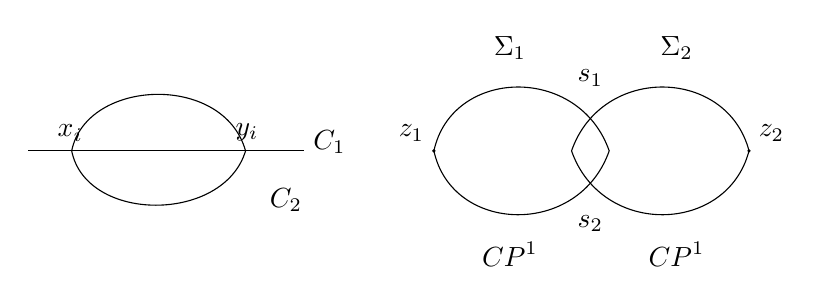
\begin{tikzpicture}[x=0.92cm,y=0.92cm]
 \draw (-5.4,0)--(-1.6,0);
 \draw (-4.8,0) .. controls (-4.6,1.00) and (-2.7,1.08) .. (-2.4,0)
                    .. controls (-2.7,-1.00) and (-4.6,-1.00) .. (-4.8,0);
 \node[above] at (-4.82,0) {$x_i$};
 \node[above] at (-2.38,0) {$y_i$};
 \node[right] at (-1.60,0.12) {$C_1$};
 \node[right] at (-2.20,-0.68) {$C_2$};

 \draw (0.20,0) .. controls (0.45,1.15) and (2.20,1.20) .. (2.62,0)
                  .. controls (2.20,-1.20) and (0.45,-1.15) .. (0.20,0);
 \draw (2.10,0) .. controls (2.52,1.20) and (4.25,1.15) .. (4.55,0)
                  .. controls (4.25,-1.15) and (2.52,-1.20) .. (2.10,0);
 \fill (0.20,0) circle (0.025) (4.55,0) circle (0.025);
 \node[above left] at (0.20,0) {$z_1$};
 \node[above right] at (4.55,0) {$z_2$};
 \node[above] at (2.36,0.76) {$s_1$};
 \node[below] at (2.36,-0.76) {$s_2$};
 \node[above] at (1.25,1.12) {$\Sigma_1$};
 \node[above] at (3.55,1.12) {$\Sigma_2$};
 \node[below] at (1.25,-1.12) {$\mathbb{CP}^1$};
 \node[below] at (3.55,-1.12) {$\mathbb{CP}^1$};
\end{tikzpicture}
\caption{刚性节点有理曲线。}
\label{fig:rigid-nodal-rational-curve}
\end{figure}

取映射序列 $u_i:(\Sigma,\boldsymbol z)\to\mathbb{CP}^2$，使两个节点像
$x_i,y_i$ 相互趋近。令 $u_{i,a}^{-1}(x_i)=s_{i,a}$、
$u_{i,a}^{-1}(y_i)=t_{i,a}$。在 $\Sigma_a\cong\mathbb{CP}^1$ 上施以
$PSL(2,\mathbb C)$，可设 $s_{i,a}=s_a,t_{i,a}=t_a$ 固定，而
\[
 \operatorname{dist}(u_{i,a}(s_a),u_{i,a}(t_a))\to0,\qquad a=1,2,
\]
因为
\[
 u_{i,a}(s_a)=x_i,\qquad u_{i,a}(t_a)=y_i.
\]
下面提出一个基本问题。

\begin{question}\label{ques:fixed-domain-rigid-nodal-limit}
能否在保持相交型 $D_0$ 的定义域 $(\Sigma,\boldsymbol z)$ 上找到一个
$C^\infty$ 收敛的 $u_i$ 序列，而其像曲线极限具有图\ref{fig:domain-four-components}所示的奇点？
\end{question}

我们断言这是不可能的，理由如下。
\begin{enumerate}[label=(\arabic*)]
 \item 若这样一个定义域上的序列 $u_i$ 收敛到极限映射
 $u_\infty=(u_{1,\infty},u_{2,\infty})$，而定义域仍在
 $\overline{\mathcal M}_{1,2}$ 中，则两个映射 $u_{a,\infty}$（$a=1,2$）
 都必须在 $s_a,t_a$ 处有奇异值。
 \item 因为 $\Sigma_a$（$a=1,2$）是刚性的，极限曲线不可能可约：这些同调类中的
 不可约曲线是嵌入曲线，所以极限也必须嵌入。特别地，它们的分歧阶在极限中必须保持不变，
 这与 (1) 矛盾。
\end{enumerate}

\begin{figure}[htbp]
\centering
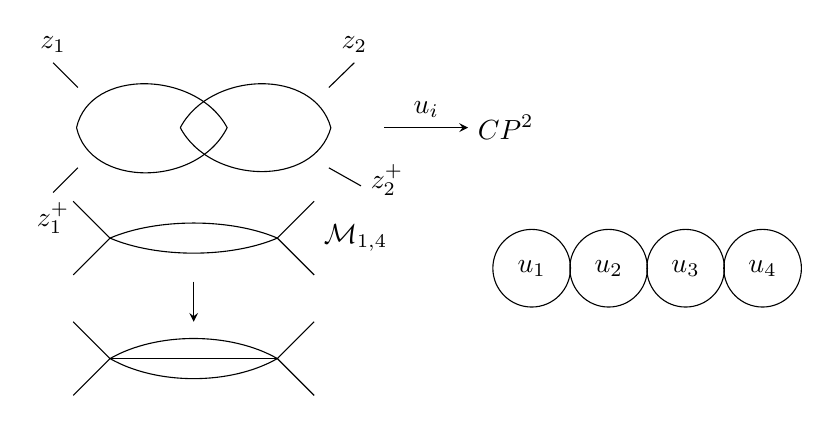
\begin{tikzpicture}[x=0.85cm,y=0.85cm,>=stealth]
 \draw (-5.7,1.55) .. controls (-5.5,2.45) and (-3.9,2.40) .. (-3.45,1.55)
                     .. controls (-3.9,0.65) and (-5.5,0.65) .. (-5.7,1.55);
 \draw (-4.15,1.55) .. controls (-3.70,2.40) and (-2.15,2.45) .. (-1.90,1.55)
                     .. controls (-2.15,0.65) and (-3.70,0.70) .. (-4.15,1.55);
 \draw (-5.68,2.15)--(-6.05,2.52) node[above] {$z_1$};
 \draw (-5.68,0.95)--(-6.05,0.58) node[below] {$z_1^+$};
 \draw (-1.93,2.15)--(-1.55,2.52) node[above] {$z_2$};
 \draw (-1.93,0.95)--(-1.45,0.68) node[right,yshift=2pt] {$z_2^+$};
 \draw[->] (-1.10,1.55)--(0.15,1.55) node[midway,above] {$u_i$};
 \node[right] at (0.15,1.55) {$\mathbb{CP}^2$};

 \coordinate (a) at (-5.2,-0.10); \coordinate (b) at (-2.7,-0.10);
 \draw (a)--++(-0.55,0.55) (a)--++(-0.55,-0.55)
       (b)--++(0.55,0.55) (b)--++(0.55,-0.55);
 \draw (a) .. controls (-4.50,0.20) and (-3.40,0.20) .. (b);
 \draw (a) .. controls (-4.50,-0.40) and (-3.40,-0.40) .. (b);
 \node[right] at (-2.15,-0.10) {$\mathcal M_{1,4}$};
 \draw[->] (-3.95,-0.75)--(-3.95,-1.35);
 \coordinate (c) at (-5.2,-1.90); \coordinate (d) at (-2.7,-1.90);
 \draw (c)--++(-0.55,0.55) (c)--++(-0.55,-0.55)
       (d)--++(0.55,0.55) (d)--++(0.55,-0.55);
 \draw (c)--(d);
 \draw (c) .. controls (-4.50,-1.50) and (-3.40,-1.50) .. (d);
 \draw (c) .. controls (-4.50,-2.30) and (-3.40,-2.30) .. (d);

 \foreach \x/\lab in {1.1/u_1,2.25/u_2,3.40/u_3,4.55/u_4}{
   \draw (\x,-0.55) circle (0.58); \node at (\x,-0.55) {$\lab$};
 }
\end{tikzpicture}
\caption{定义域。}
\label{fig:domain-four-components}
\end{figure}

从这个例子得到的教训是：这个特定稳定映射（记为 $\tau$）的像，不可能是定义域
$(\Sigma,\boldsymbol z)$ 保持固定相交型 $D_0$ 的稳定映射的极限之像；它必须与另一个
定义域具有不同相交型的稳定映射有相同的像。

现在说明这个例子中真正发生的事情。考虑 $((\Sigma,\boldsymbol z),u_i)$，其像形如
$C_{1,i}\cup C_{2,i}$。我们想描述收敛
\[
 ((\Sigma,\boldsymbol z),u_i)\longrightarrow
 ((\Sigma,\boldsymbol z),u_\infty)
 \quad\text{于 }\overline{\mathcal M}_{1,2}(\mathbb{CP}^2,3[H]).
\]
注意，在上述不恰当的收敛论证中，$u_i:(\Sigma,\boldsymbol z)\to\mathbb{CP}^2$
的定义域是稳定的，但预期极限映射的定义域不稳定。为了定义正确的收敛概念，需要在每个分支
上再添一个标记点，使映射 $u_2,u_3$ 收敛到 $C_1\cap C_2$ 中一点处的常值映射。
随后遗忘新增标记点，就得到所需极限。该极限有四个而非两个不可约分支，其中两个是定义域稳定的
常值分支。

为系统处理上述不稳定性问题，我们采用添加额外标记点的方法。这既用来稳定定义域，也用来正确
编码冒泡现象。我们先给出序列收敛的定义，最后再给出相应拓扑的一组基。
\end{example}

\textbf{I. 稳定情形。}
\stfhIndex{I031}{00-symbol-031}{$\overline{\mathcal M}^{st}_{g,m}(M,J;\beta)$}
\stfhIndex{I033}{00-symbol-033}{$\widetilde{\mathcal M}_{g,m}(M,J;\beta)$}
\stfhIndex{I034}{00-symbol-034}{$\widetilde{\mathcal M}^{st}_{g,m}(M,J;\beta)$}
以
$\overline{\mathcal M}_{g,m}^{st}(M,J;\beta)
\subset\overline{\mathcal M}_{g,m}(M,J;\beta)$
表示定义域稳定的稳定映射之（等价类）子集。以
$\widetilde{\mathcal M}_{g,m}(M,J;\beta)$ 和
$\widetilde{\mathcal M}_{g,m}^{st}(M,J;\beta)$
分别表示\emph{稳定映射}的集合以及其中\emph{定义域}稳定者的集合，而不只是等价类。我们先借助
$\widetilde{\mathcal M}_{g,m}^{st}(M,J;\beta)$ 中稳定映射的序列收敛，定义
$\overline{\mathcal M}_{g,m}^{st}(M,J;\beta)$ 上序列收敛的意义；最后再给出相应拓扑的基。

设 $\mathbf x=[(\Sigma,\boldsymbol z),u]$，其相交型为
$D=(T,\{g_v\},o,\{\beta_v\})$；考虑稳定映射序列
$((\Sigma_i,\boldsymbol z_i),u_i)$。由于固定 $\beta$ 的相交型只有有限多个，取子列后可设其相交型恒为同一个
$D$。由
$\overline{\mathcal M}_{g,m}$ 拓扑的定义，存在另一相交型
$D'$，使得或者 $D'=D$，或者可将稳定曲线
$(\Sigma_i,\boldsymbol z_i)$ 表示为
\[
 (\Sigma_i,\boldsymbol z_i)=
 \operatorname{Res}_{(\Sigma_i',\boldsymbol z_i')}
 (\{\alpha_{e,i}\}_{e\in E_T}),
\]
其中
$[\Sigma_i',\boldsymbol z_i']\to[\Sigma,\boldsymbol z]$ 于
$\mathcal M_{g,m}^D$，且 $\alpha_{e,i}\to0$；这里在奇点处给定的充分小粘合参数满足
\[
 (\alpha_{e,i})_{e\in E_T}\in
 \bigoplus_{e=[v,w]}T_{x_{v,i}}\Sigma_{v,i}'\otimes
 T_{x_{w,i}}\Sigma_{w,i}'.
\]
令
$R_{e,i}^{-1/2}=|\alpha_{e,i}|$。按例 9.4.21 的度量，在每个节点定义颈部
以前，先回忆：按定义，$\Sigma_i$ 有一个子集可与
\[
 \Sigma_i'\setminus\bigcup_{x_{v,i}}D_{x_{v,i}}(R_{e,i}^{-3/2})
\]
识别；而对于例 9.4.21 所显式给出的度量，有
\[
 \operatorname{diam}\!\left(
 \Sigma_i\setminus\left(
 \Sigma_i'\setminus\bigcup_{x_{v,i}}D_{x_{v,i}}(R_{e,i}^{-3/2})
 \right)\right)\longrightarrow0
 \qquad(i\to\infty).
\]
给定 $\mu>0$ 及一族充分大的 $R_{e,i}$，在节点
$x_{e,i}=(x_{v,i},x_{w,i})\in\operatorname{Sing}(\Sigma_i)$ 处定义指定的颈部
\[
 W_{e,i}(\mu)=
 (D_{x_{v,i}}(\mu)\setminus D_{x_{v,i}}(R_{e,i}^{-1}))
 \cup
 (D_{x_{w,i}}(\mu)\setminus D_{x_{w,i}}(R_{e,i}^{-1})),
 \qquad W_i(\mu)=\bigcup_eW_{e,i}(\mu).
\]
见图\ref{fig:resolution-stable-domain}。

\begin{figure}[htbp]
\centering
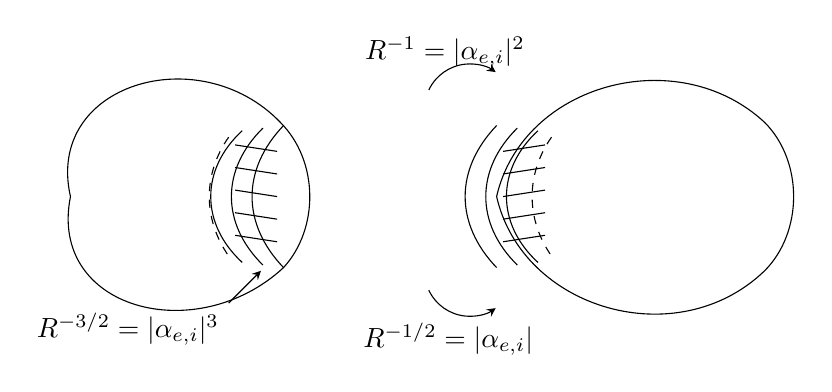
\begin{tikzpicture}[x=0.82cm,y=0.82cm,>=stealth]
 \draw (-5.4,0) .. controls (-5.8,1.75) and (-3.4,2.45) .. (-2.15,1.15)
                 .. controls (-1.55,0.55) and (-1.55,-0.50) .. (-2.10,-1.10)
                 .. controls (-3.45,-2.35) and (-5.75,-1.75) .. (-5.4,0);
 \draw (1.20,0) .. controls (1.60,1.75) and (4.00,2.40) .. (5.35,1.15)
                 .. controls (5.95,0.55) and (5.95,-0.55) .. (5.35,-1.15)
                 .. controls (4.00,-2.45) and (1.60,-1.75) .. (1.20,0);
 \draw (-2.10,1.10) .. controls (-2.75,0.42) and (-2.75,-0.42) .. (-2.10,-1.10);
 \draw (-2.42,1.06) .. controls (-3.07,0.42) and (-3.07,-0.42) .. (-2.42,-1.06);
 \draw (-2.74,1.02) .. controls (-3.39,0.42) and (-3.39,-0.42) .. (-2.74,-1.02);
 \draw (1.20,1.10) .. controls (0.55,0.42) and (0.55,-0.42) .. (1.20,-1.10);
 \draw (1.52,1.06) .. controls (0.87,0.42) and (0.87,-0.42) .. (1.52,-1.06);
 \draw (1.84,1.02) .. controls (1.19,0.42) and (1.19,-0.42) .. (1.84,-1.02);
 \draw[dashed] (-2.95,0.92) .. controls (-3.35,0.35) and (-3.35,-0.35) .. (-2.95,-0.92);
 \draw[dashed] (2.05,0.92) .. controls (1.65,0.35) and (1.65,-0.35) .. (2.05,-0.92);
 \foreach \y in {-0.70,-0.35,0,0.35,0.70}{
   \draw (-2.85,{\y+0.10})--(-2.20,\y);
   \draw (1.30,\y)--(1.95,{\y+0.10});
 }
 \draw[->] (0.15,1.65) arc[start angle=155,end angle=55,radius=0.70];
 \node[above] at (0.40,1.85) {$R^{-1}=|\alpha_{e,i}|^2$};
 \draw[->] (-2.95,-1.65)--(-2.45,-1.15);
 \node[below left] at (-2.95,-1.65) {$R^{-3/2}=|\alpha_{e,i}|^3$};
 \draw[->] (0.15,-1.45) arc[start angle=205,end angle=305,radius=0.70];
 \node[below] at (0.45,-1.80) {$R^{-1/2}=|\alpha_{e,i}|$};
\end{tikzpicture}
\caption{解节点。}
\label{fig:resolution-stable-domain}
\end{figure}

\begin{definition}\label{def:stable-domain-sequential-convergence}
\stfhIndex{I245}{xu^lie^shou^lian}{序列收敛（sequential convergence）}
记
$\operatorname{s-lim}_{i\to\infty}[(\Sigma_i,\boldsymbol z_i),u_i]
=[(\Sigma,\boldsymbol z),u]$，如果：
\begin{enumerate}[label=(\arabic*)]
 \item $[\Sigma_i,\boldsymbol z_i]\to[\Sigma,\boldsymbol z]$ 于
 $\overline{\mathcal M}_{g,m}$；
 \item 对任意 $\mu>0$，$u_i|_{\Sigma_i'\setminus W_{e,i}(\mu)}$ 在紧子集上以
 $C^\infty$ 收敛到 $u$；
 \item 对每个节点 $x_e$，
 \[
  \lim_{\mu\to0}\left(\limsup_{i\to\infty}
  \operatorname{diam}(u_i(W_{e,i}(\mu)))\right)=0.
 \]
\end{enumerate}
\end{definition}

\stfhIndex{I061}{wu^qiong^yuan^chu^de^ta^pu^ji}{无穷远处的拓扑基（basis of topology at infinity）}
条件 (1) 的含义是可选代表使定义域按命题 9.3.19 和定理 9.4.27 的意义收敛。现在把这一定义改写为\emph{无穷远处的邻域基}。记稳定曲线
$\mathbf v=[\Sigma,\boldsymbol z]$、稳定映射
$\mathbf x=[(\Sigma,\boldsymbol z),u]$。存在节点集的邻域
$\mathcal U(\operatorname{Sing}(\Sigma))$，以及典范光滑嵌入
\begin{equation}
 i_{\mathbf v}:\Sigma\setminus\mathcal U(\operatorname{Sing}(\Sigma))
 \longrightarrow\operatorname{Res}_{(\Sigma,\boldsymbol z)}
 (\{\alpha_e\}_{e\in E_T}),
 \label{eq:canonical-embedding-resolved-domain}
\end{equation}
使 $i_{\mathbf v}(z_i)=z_i$，并可设其在上述邻域外全纯。给
$\overline{\mathcal M}_{g,m}$ 选取适当度量并在其上定义距离；回忆
$\overline{\mathcal M}_{g,m}$ 是 orbifold (DM69)，且可赋黎曼度量。以
$\mathfrak U(\mathbf v)$ 表示 $\mathbf v$ 的邻域。

\begin{definition}\label{def:stable-domain-neighborhood}
给定 $\mathbf x$ 与 $\epsilon>0$，定义满足下列条件的稳定映射
$\mathbf x'=((\Sigma',\boldsymbol z'),u')$ 的集合：
\begin{enumerate}[label=(\arabic*)]
 \item $\mathbf v'=(\Sigma',\boldsymbol z')\in\mathfrak U(\mathbf v)$，且
 $\operatorname{dist}(\mathbf v',\mathbf v)<\epsilon$；
 \item 存在双全纯映射 $\varphi$，使在
 $\Sigma\setminus\mathcal U(\operatorname{Sing}(\Sigma))$ 上，
 $u'\circ i_{\mathbf v\mathbf v'}$ 与 $u\circ\varphi$ 的 $C^1$ 距离小于 $\epsilon$；
 \item 若 $S$ 是
 $\Sigma'\setminus i_{\mathbf v\mathbf v'}(\Sigma\setminus
 \mathcal U(\operatorname{Sing}(\Sigma)))$ 的任一连通分支，则
 $\operatorname{diam}(u'(S))<\epsilon$。
\end{enumerate}
\end{definition}

\begin{lemma}\label{lem:stable-domain-topology-basis}
由定义\ref{def:stable-domain-neighborhood}中的稳定映射同构类组成的集合
$\mathcal U^{st}(\epsilon,\mathbf x)$，构成
$\overline{\mathcal M}_{g,m}^{st}(M,J;\beta)$ 上一个拓扑的基。
\end{lemma}

\begin{exercise}\label{ex:stable-domain-topology-basis}
证明此引理。
\end{exercise}

\textbf{II. 一般情形。}
一般稳定映射的定义域未必稳定。给定序列，依次：增加有限个标记点
$\boldsymbol w_i$ 使定义域稳定；按上述 $\operatorname{s-lim}$ 取极限；最后遗忘新增标记点。

\begin{definition}\label{def:general-stable-map-convergence}
\stfhSubIndex{I262}{wen^ding^ying^she^ta^pu}{稳定映射拓扑（stable map topology）}{ding^yi}{定义（definition）}
设 $[(\Sigma_i,\boldsymbol z_i),u_i]$ 与
$[(\Sigma,\boldsymbol z),u]$ 属于
$\overline{\mathcal M}_{g,m}(M,J;\beta)$。称
\[
 \lim_{i\to\infty}[(\Sigma_i,\boldsymbol z_i),u_i]
 =[(\Sigma,\boldsymbol z),u],
\]
若存在稳定曲线
$(\Sigma_i,\boldsymbol z_i^+)$，其中
$\boldsymbol z_i^+=\boldsymbol z_i\cup\boldsymbol w_i$ 且
$\#\boldsymbol w_i=n$，以及稳定极限
$((\Sigma_\infty,\boldsymbol z_\infty^+),u_\infty)$，使
\begin{enumerate}[label=(\arabic*)]
 \item
 $\operatorname{s-lim}_{i\to\infty}
 [((\Sigma_i,\boldsymbol z_i^+),u_i)]
 =[((\Sigma_\infty,\boldsymbol z_\infty^+),u_\infty)]$；
 \item
 $\operatorname{forget}_{m+n;n}
 [((\Sigma_\infty,\boldsymbol z_\infty^+),u_\infty)]
 =[((\Sigma,\boldsymbol z),u)]$。
\end{enumerate}
\end{definition}

遗忘映射会把遗忘标记点后变成不稳定、且其上映射恒定的分支收缩为一点。下面构造与这种序列收敛相伴的拓扑。对
$\mathbf x=[(\Sigma,\boldsymbol z),u]$ 的一个代表，选择有限标记点
$\boldsymbol w=(w_a)_{a\in A}$，$\ell=\#A$，要求：

\begin{condition}\label{cond:additional-marked-points}
\begin{enumerate}[label=(\arabic*)]
 \item $\boldsymbol w$ 与 $\boldsymbol z$ 及 $\Sigma$ 的节点集不交；
 \item $(\Sigma,\boldsymbol w)$ 稳定，且无非平凡自同构；
 \item $u$ 在每个 $w_a$ 处是浸入。
\end{enumerate}
\end{condition}

总能作出这种选择。令
$\mathbf v=[\Sigma,\boldsymbol z\cup\boldsymbol w]
\in\overline{\mathcal M}_{g,m+\ell}$，取邻域
$\mathfrak U(\mathbf v)$。存在节点集邻域 $\mathcal U(S(\Sigma))$，使任意
$\mathbf v'=[\Sigma',\boldsymbol z'\cup\boldsymbol w']\in\mathfrak U(\mathbf v)$
都有连续依赖于 $\mathbf v'$ 的光滑嵌入
\begin{equation}
 i_{\mathbf v\mathbf v'}:\Sigma\setminus\mathcal U(S(\Sigma))\longrightarrow\Sigma',
 \label{eq:embedding-stabilized-nearby-domain}
\end{equation}
满足
\begin{equation}
 i_{\mathbf v\mathbf v'}(z_i)=z_i,\qquad i_{\mathbf v\mathbf v'}(w_a)=w_a,
 \label{eq:embedding-preserves-marked-points}
\end{equation}
并可设其在节点邻域外全纯；还要求 $i_{\mathbf v\mathbf v'}$ 在 $C^\infty$ 意义下连续依赖于
$\mathbf v'$。

对每个 $w_a$，选取法向切片 $N_{w_a}$，满足：
\begin{condition}[法向切片]\label{cond:normal-slices}
\begin{enumerate}[label=(\arabic*)]
 \item $N_{w_a}$ 是余维 $2$ 的光滑子流形；
 \item $N_{w_a}$ 在 $u(w_a)$ 处横截于 $u(\Sigma)$。
\end{enumerate}
\end{condition}

这些切片只依赖固定的代表
$\overline{\mathbf x}=((\Sigma,\boldsymbol z),u)$ 和
$\boldsymbol w=\{w_a\}_{a\in A}$；一旦给定后二者，便\emph{一劳永逸地固定}这些切片。
它们还带有由环境空间 $M$ 的度量诱导的度量。为
$\overline{\mathcal M}_{g,\ell+m}$ 配备一个适当度量，以定义
$\mathbf v'$ 与 $\mathbf v$ 之间的距离。

\begin{definition}[稳定化]\label{def:stabilization-neighborhood-general-case}
给定 $\mathbf x$、代表 $\overline{\mathbf x}=((\Sigma,\boldsymbol z),u)$ 以及
$\epsilon_1,\epsilon_2>0$，令
$\mathcal V(\epsilon_1,\epsilon_2,\overline{\mathbf x})$ 为满足下列条件的稳定映射
$\overline{\mathbf x}'=((\Sigma',\boldsymbol z'),u')$ 的集合：
\begin{enumerate}[label=(\arabic*)]
 \item $\mathbf v'=[\Sigma',\boldsymbol z'\cup\boldsymbol w']
 \in\mathfrak U(\mathbf v)$ 且
 $\operatorname{dist}(\mathbf v',\mathbf v)<\epsilon_1$；
 \item 存在双全纯映射 $\varphi$，使
 $u'\circ i_{\mathbf v\mathbf v'}$ 与 $u\circ\varphi$ 在节点邻域外的
 $C^1$ 距离小于 $\epsilon_1$；
 \item 对补集任一连通分支 $S$，$\operatorname{diam}(u'(S))<\epsilon_1$；
 \item 写 $\boldsymbol w'=(w_a')_{a\in A}$，要求
 $u'(w_a')\in N_{w_a}$，且
 \[
  \operatorname{dist}(u'(w_a'),u(\varphi(w_a)))<\epsilon_2.
 \]
\end{enumerate}
称 $\overline{\mathbf x}'$ 关于 $\boldsymbol w$ 与
$\overline{\mathbf x}$ 是 $(\epsilon_1,\epsilon_2)$-接近的。
\end{definition}

当 $\epsilon_1,\epsilon_2$ 充分小时，横截性使 $\boldsymbol w'$ 由
$\boldsymbol w,N_{w_a}$ 唯一确定。一方面，我们引入有限多个额外标记点
$\boldsymbol w'=\{w_a'\}$；另一方面，也引入同样数目的余维 $2$ 条件
\begin{equation}
 u'(w_a')\in N_{w_a},
 \label{eq:normal-slice-incidence-condition}
\end{equation}
故虚维数保持不变。定义
\begin{equation}
 \mathfrak U(\mathbf x;\epsilon_1,\epsilon_2)
 =\{[((\Sigma',\boldsymbol z'),u')]\mid
 ((\Sigma',\boldsymbol z'),u')
 \in\mathcal V(\epsilon_1,\epsilon_2,\overline{\mathbf x})\},
 \label{eq:general-stable-map-neighborhood}
\end{equation}
它是来自 $\mathcal V(\epsilon_1,\epsilon_2,\overline{\mathbf x})$ 的元素之等价类集合。
若记
\[
 \mathcal V^{st}(\epsilon_1,\epsilon_2,
 \overline{\mathbf x};\boldsymbol w(\overline{\mathbf x}))
 :=\{((\Sigma',\boldsymbol z'\cup\boldsymbol w'),u')
 \mid ((\Sigma',\boldsymbol z'),u')
 \in\mathcal V(\epsilon_1,\epsilon_2,\overline{\mathbf x})\},
\]
并把它在
$\overline{\mathcal M}_{g,m+n}^{st}(M,J;\beta)$ 中的投影记为
$\mathcal U^{st}(\epsilon_1,\epsilon_2,
\overline{\mathbf x};\boldsymbol w(\overline{\mathbf x}))$，则也可写成
\begin{equation}
 \mathfrak U(\mathbf x;\epsilon_1,\epsilon_2)
 =\operatorname{forget}_{m+n;m}
 \bigl(\mathcal U^{st}(\epsilon_1,\epsilon_2;
 \overline{\mathbf x},\boldsymbol w(\overline{\mathbf x}))\bigr).
 \label{eq:general-neighborhood-forgetful-image}
\end{equation}
由于要求 $(\Sigma,\boldsymbol w(\overline{\mathbf x}))$ 的自同构群平凡，
$\mathcal V^{st}(\epsilon_1,\epsilon_2,
\overline{\mathbf x};\boldsymbol w(\overline{\mathbf x}))$ 到
$\overline{\mathcal M}_{g,m+n}^{st}(M,J;\beta)$ 的投影是单射。

\begin{proposition}\label{prop:stable-map-topology-neighborhood-basis}
当 $\mathbf x$ 与 $\epsilon_1,\epsilon_2>0$ 变化时，集合族
$\mathfrak U(\mathbf x;\epsilon_1,\epsilon_2)$ 构成
$\overline{\mathcal M}_{g,m}(M,J;\beta)$ 上一个拓扑的基；而且该拓扑不依赖构造中
$\boldsymbol w$ 与 $N_{w_a}$ 的选择。
\end{proposition}

\begin{exercise}\label{ex:stable-map-topology-equivalent-sequential}
证明此命题，并证明所得拓扑等价于上面由序列收敛诱导的拓扑。
\end{exercise}

\subsection{紧性}
\label{subsec:stable-map-compactness}
\stfhSubIndexRangeStart{I261}{wen^ding^ying^she^ta^pu}{稳定映射拓扑（stable map topology）}{jin^xing}{紧性（compactness）}

本小节证明稳定映射拓扑的紧性。

\begin{theorem}\label{thm:gromov-compactness-stable-maps}
$\overline{\mathcal M}_{g,m}(M,\omega,J;\beta)$ 是紧的。
\end{theorem}

证明按\eqref{eq:general-neighborhood-forgetful-image}中的邻域基或定义
\ref{def:general-stable-map-convergence}的序列收敛分成若干步骤。还要注意，稳定映射空间中
有三种导致收敛失效的来源：
\begin{enumerate}[label=(\arabic*)]
 \item 映射在某些不稳定分支上趋于常值；
 \item 两个或更多标记点发生碰撞；
 \item 导数爆破，即对某列 $z_i$ 有 $|du_i(z_i)|\to\infty$。
\end{enumerate}

\textbf{定义域的初始稳定化。}
给定稳定映射序列 $((\Sigma_i,\boldsymbol z_i),u_i)$。由相交型有限性，取子列后可设它们都属于固定的层
$\mathcal M_{g,m}^D(M,J;\beta)$。加入\emph{同样数目} $n=\#A$ 的标记点
$\boldsymbol w_i=\{w_{i,a}\}_{a\in A}$，令
$\boldsymbol z_i^+=\boldsymbol z_i\cup\boldsymbol w_i$，使
$(\Sigma_i,\boldsymbol z_i^+)$ 稳定。由
$\overline{\mathcal M}_{g,m+n}$ 的紧性，再取子列使
\begin{equation}
 \lim_{i\to\infty}(\Sigma_i,\boldsymbol z_i^+)
 =(\Sigma_\infty^+,\boldsymbol z_\infty^+).
 \label{eq:initial-stabilized-domain-limit}
\end{equation}
记极限的相交型为 $D^+=(T^+,\{g_v^+\},o^+)$。把
$\Sigma_\infty^+=\bigcup_v\Sigma_{\infty,v}$ 分解为不可约分支。按
\eqref{eq:initial-stabilized-domain-limit}的收敛定义，
\[
 (\Sigma_i,\boldsymbol z_i^+)=
 \operatorname{Res}_{(\Sigma_i',\boldsymbol z_i^{\prime+})}
 (\{\alpha_{e,i}\}),
 \qquad \alpha_{e,i}\to0,
\]
且
\begin{equation}
 \lim_{i\to\infty}(\Sigma_i',\boldsymbol z_i^{\prime+})
 =(\Sigma_\infty^+,\boldsymbol z_\infty^+)
 \quad\text{于 }\mathcal M_{g,m+n}^{D^+}.
 \label{eq:fixed-stratum-stabilized-domain-limit}
\end{equation}
由\eqref{eq:fixed-stratum-stabilized-domain-limit}中的收敛，可取只依赖极限曲面的统一常数 $\epsilon_0>0$ 和各节点附近的复坐标，使
$z(U_{x_v})\supset D^2(\epsilon_0)$。

\begin{remark}\label{rem:metrics-stabilized-domains}
稳定定义域并取极限的实质，是抽取 $\Sigma_i,\Sigma_i'$ 上的一列度量，使其按深谷--小野形变、尤其按颈部附近的规定，收敛到
$\Sigma_\infty^+$ 上的度量。这使我们可以在远离极限奇点的任意紧集上研究 $u_i$ 的 $C^1$ 收敛。
\end{remark}

\textbf{远离颈部区域的收敛。}
以深谷--小野形变可写
\[
 \Sigma_i=\operatorname{Res}_{(\Sigma_i',\boldsymbol z_i^{\prime+})}
 (\{\alpha_{x_v,i}\}),
\]
它含有一个子集，即 $i_{\mathbf v_i^{\prime+},\mathbf v_i}$ 的像，可与
\[
 \Sigma_i'\setminus\bigcup_{x_{v,i}}D_{e,i}(R_{e,i}^{-3/2})
 \subset\Sigma_i
\]
识别。这里记
$\mathbf v_i^{\prime+}=(\Sigma_i',\boldsymbol z_i^{\prime+})$、
$\mathbf v_i=(\Sigma_i,\boldsymbol z_i^+)$，并令
$R_{e,i}=|\alpha_{x_v,i}|^{-1/2}$。

\begin{proposition}\label{prop:derivative-bound-away-necks}
给定任意 $0<\mu<\epsilon_0$。在初始稳定化所选标记点的基础上再增加标记点并取子列后，存在与 $i$ 无关（可依赖 $\mu$）的常数 $C>0$，使
\[
 \sup_{\Sigma_i'\setminus\bigcup_{x_{v,i}}D_{x_{v,i}}(\mu)}|du_i|
 \le C.
\]
\end{proposition}

\begin{figure}[htbp]
\centering
\setlength{\unitlength}{0.8mm}
\begin{picture}(125,42)
 \qbezier(7,38)(40,5)(66,17)
 \qbezier(66,17)(91,28)(119,39)
 \qbezier(8,2)(37,35)(65,23)
 \qbezier(65,23)(91,12)(120,1)
 \put(65,20){\oval(4,6)[r]}
\end{picture}
\caption{细颈部。}
\label{fig:thin-neck}
\end{figure}

在证明命题 9.5.28 前回忆几个将用于证明的引理；下面这个衰减估计的证明将在附录 B 给出。

\begin{lemma}\label{lem:exponential-decay-long-cylinder}
存在 $L_0>0$、$\epsilon_1>0$，使得对任意 $L\ge L_0$，若
$u:[-L-1,L+1]\times S^1\to(M,J)$ 是 $J$-全纯的，且
$\operatorname{diam}(u([-L-1,L+1]\times S^1))\le\epsilon_1$，则
\[
 \left|\frac{\partial u}{\partial\tau}(\tau,t)\right|
 +\left|\frac{\partial u}{\partial t}(\tau,t)\right|
 \le Ce^{-\lambda\operatorname{dist}(\tau,\partial[-L-1,L+1])}
\]
对 $(\tau,t)\in[-L,L]\times S^1$ 成立；其中 $\lambda,C>0$ 与
$L\ge L_0$ 无关。
\end{lemma}

粗略地说，这个引理断言：若定义在长圆柱上的 $J$-全纯映射之像的直径充分小，
则其像看起来像图\ref{fig:thin-neck}中的双曲曲面。这个指数估计立即给出下面关于
$\mathbb C$ 中环带上所定义的 $J$-全纯映射的导数估计。

\begin{corollary}\label{cor:derivative-estimate-holomorphic-annulus}
考虑共形等同
\[
 [-L,L]\times S^1\cong\operatorname{Ann}(r,1),
 \qquad w\longmapsto e^{-L}e^w,\qquad r=e^{-2L}.
\]
若 $z$ 是 $D^2(1)\subset\mathbb C$ 的标准复坐标，则
\[
 \left|\frac{\partial u}{\partial z}(z)\right|
 +\left|\frac{\partial u}{\partial\overline z}(z)\right|
 \le C\lambda\max\left(1,\frac r{|z|^2}\right)
\]
对所有满足
$\log|z|\in[\log r+1,\log r-1]$ 的 $z$ 成立（即在略缩小的环带上）。
\end{corollary}

\begin{proof}[命题 9.5.28 的证明]
令 $\epsilon_1$ 为引理\ref{lem:exponential-decay-long-cylinder}中的常数。给定 $\mu>0$，取子列后可设每个分支满足二者之一：
\begin{equation}
 \operatorname{diam}u_i(\Sigma_{i,v}'\setminus
 \bigcup_{x_{v,i}}D_{x_{v,i}}(\mu))\ge\frac{\epsilon_1}{1000},
 \label{eq:thick-component-threshold}
\end{equation}
或
\begin{equation}
 \operatorname{diam}u_i(\Sigma_{i,v}'\setminus
 \bigcup_{x_{v,i}}D_{x_{v,i}}(\mu))\le\frac{\epsilon_1}{100}.
 \label{eq:thin-component-threshold}
\end{equation}
称前者为\emph{厚}分支，后者为\emph{薄}分支；两类不互斥但覆盖全部分支。薄分支由引理 9.5.29 满足命题所需估计。

先分析厚分支，记厚分支集合为
\[
 V_{1,i}=V_1((\Sigma_i,\boldsymbol z_i^+),u_i)
 :=\left\{v\in V_T\ \middle|\
 \operatorname{Diam}u_i\!\left(\Sigma_{i,v}'\setminus
 \bigcup_{x_{v,i}}D_{x_{v,i}}(\mu)\right)\ge\frac{\epsilon_1}{1000}
 \right\}.
\]
由单调性公式，若 $v\in V_{1,i}$，则
\[
 \operatorname{Area}\!\left(\Sigma_{i,v}'\setminus
 \bigcup_{x_{v,i}}D_{x_{v,i}}(\mu)\right)
 =\int_{\Sigma_{i,v}'\setminus\bigcup_{x_{v,i}}D_{x_{v,i}}(\mu)}u_i^*\omega
 \ge C\epsilon_1^2.
\]
故 $\#V_{1,i}$ 有与 $i$ 及 $\Sigma_i^+$ 上新增标记点数无关的统一上界。再定义
\begin{equation}
 \begin{split}
 V_{2,i}:={}&\{v\in V_{1,i}\mid
 \exists z_{a,j_1},z_{a,j_2}\in\Sigma_{i,v}\cap\boldsymbol z_i^+,\\
 &\hspace{33mm}
 \operatorname{dist}(u_i(z_{a,j_1}),u_i(z_{a,j_2}))
 \ge\epsilon_1/1000\},
 \end{split}
 \label{eq:marked-image-separated-components}
\end{equation}
以及
\begin{equation}
 V_{3,i}:=\{v\in V_{1,i}\mid
 \limsup_{i\to\infty}
 \sup_{\Sigma_{i,v}'\setminus\bigcup D_{x_{v,i}}(\mu)}|du_i|<\infty\}.
 \label{eq:bounded-derivative-components}
\end{equation}
显然 $\#V_{2,i},\#V_{3,i}\le\#V_{1,i}$。

\begin{lemma}\label{lem:marked-points-increase-complexity}
若存在点
$p_i\in\Sigma_i'\setminus\bigcup_{x_{v,i}}D_{x_{v,i}}(\mu)
=(\Sigma_i\setminus\bigcup_{e\in E_T}W_e(\mu))$，使
$|du_i(p_i)|\to\infty$；特别地，$v\in V_{1,i}$。则取子列、增加标记点并为
$(\Sigma_i,\boldsymbol z_i^{++})$ 取新极限后，下列之一成立：
\begin{enumerate}[label=(\arabic*)]
 \item $\#V_1((\Sigma_i,\boldsymbol z_i^{++}),u_i)>
 \#V_1((\Sigma_i,\boldsymbol z_i^+),u_i)$；
 \item $\#V_1$ 不变而 $\#V_2$ 增加；
 \item $\#V_1,\#V_2$ 不变而 $\#V_3$ 增加。
\end{enumerate}
\end{lemma}

\begin{proof}
记正则部分为
$\Sigma_{i,v}'(\mu;\mathrm{reg})=
\Sigma_{i,v}'\setminus\bigcup D_{x_{v,i}}(\mu)$，取 $p_i$ 使
$|du_i(p_i)|$ 达到其上确界 $C_{v,i}$。分两种情形：
\[
 C_{v,i}\operatorname{dist}(p_i,\partial\Sigma_{i,v}'(\mathrm{reg}))
 \to\infty,
 \qquad\text{或}\qquad
 C_{v,i}\operatorname{dist}(p_i,\partial\Sigma_{i,v}'(\mathrm{reg}))
 \to D_v\ge0.
\]
第一种情形中，按 $C_{v,i}$ 的量级重标度定义域，由冒泡论证在 $p_i$ 附近产生一个气泡。
特别地，可选 $p_i'$ 使
$\operatorname{dist}(u_i(p_i),u_i(p_i'))\ge\epsilon_1/2$ 且
$\operatorname{dist}(p_i,p_i')<1/(2C_{v,i})$。把二者加入
$\Sigma_{i,v}'\setminus\bigcup D_{x_{v,i}}(\mu)$ 作为新标记点，并在
$\overline{\mathcal M}_{g,|\boldsymbol z_i^{++}|}$ 中考察
$(\Sigma_i,\boldsymbol z_i^{++})$ 及其极限；这里回忆，$\Sigma_i$ 含有同
$\Sigma_{i,v}'\setminus\bigcup D_{x_{v,i}}(\mu)$ 等同的子集。

由于 $p_i$ 实现了 $|du_i|$ 在 $\Sigma_{i,v}'(\mu;\mathrm{reg})$ 上的最大值，
冒泡构造说明新极限的气泡分支上有
\[
 \sup_{\Sigma_{i,v}'(\mu;\mathrm{reg})}|\nabla u_i|<C.
\]
另一方面，冒泡构造局限在 $p_i,p_i'$ 附近，故除
$\Sigma_{i,v}'\setminus\bigcup D_{x_{v,i}}(\mu)$ 外，
$\Sigma_i'$ 的所有其他分支上 $|du_i|$ 的行为都不变。因此
\[
 \#V_1((\Sigma_i,\boldsymbol z_i^+),u_i)
 \le\#V_1((\Sigma_i,\boldsymbol z_i^{++}),u_i),
\]
并且下列两个不等式之一成立：
\[
 \#V_2((\Sigma_i,\boldsymbol z_i^+),u_i)
 <\#V_2((\Sigma_i,\boldsymbol z_i^{++}),u_i)
\]
或
\[
 \#V_3((\Sigma_i,\boldsymbol z_i^+),u_i)
 <\#V_3((\Sigma_i,\boldsymbol z_i^{++}),u_i).
\]
这就完成了第一种情形的证明。

第二种情形中，
$|du_i(p_i)|\operatorname{dist}(p_i,W_{e,i}(\mu))\to D_v<\infty$。
由于 $p_i$ 趋近颈部区域的速度快于冒泡速度，通常的重标度不能完整捕获冒泡；
但仍可用引理 9.5.29 的衰减估计证明下面的子引理。

\begin{sublemma}\label{lem:two-nearby-points-separated-images}
设 $\Sigma_{i,v}'$ 是包含 $p_i$ 的分支。取子列后可选
$p_{i,+},p_{i,-}\in\Sigma_{i,v}'$，使
\begin{enumerate}[label=(\arabic*)]
 \item $\operatorname{dist}(u_i(p_{i,+}),u_i(p_{i,-}))>\epsilon_1/10$；
 \item $\operatorname{dist}(p_{i,\pm},p_i)\to0$。
\end{enumerate}
\end{sublemma}

\begin{proof}
取 $q_i\ne p_i$，$d(p_i,q_i)=\delta_i\to0$。固定足够小的
$0<\lambda<\mu$。断言
\begin{equation}
 \limsup_{i\to\infty}
 \operatorname{Diam}(u_i(D_{q_i}(\lambda)))\ge\epsilon_1/2.
 \label{eq:image-diameter-near-neck}
\end{equation}
否则取以 $q_i=0$ 为中心的复坐标，并考察
\[
 \psi_i:\operatorname{Ann}(\delta_i^2,1)\to D_{q_i}(\lambda),
 \qquad \psi_i(z)=q_i+\frac\lambda2z=\frac\lambda2z.
\]

\begin{figure}[htbp]
\centering
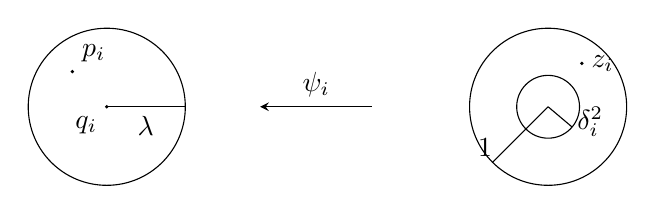
\begin{tikzpicture}[x=0.95cm,y=0.95cm,>=stealth]
 \draw (-4.30,0) circle (1.05);
 \fill (-4.76,0.47) circle (0.025) node[above right] {$p_i$};
 \fill (-4.30,0) circle (0.025) node[below left] {$q_i$};
 \draw (-4.30,0)--(-3.25,0);
 \node[below] at (-3.78,0) {$\lambda$};

 \draw[<-] (-2.25,0)--(-0.75,0) node[midway,above] {$\psi_i$};

 \draw (1.60,0) circle (1.05);
 \draw (1.60,0) circle (0.42);
 \draw (1.60,0)--(0.86,-0.74);
 \node[left] at (0.98,-0.55) {$1$};
 \draw (1.60,0)--(1.92,-0.27);
 \node[right] at (1.86,-0.20) {$\delta_i^2$};
 \fill (2.05,0.58) circle (0.025) node[right] {$z_i$};
\end{tikzpicture}
\caption{映射 $\psi_i$。}
\label{fig:map-psi-i}
\end{figure}

此时 $p_i$ 位于 $\psi_i$ 的像中。若写
$\psi_i(z_i)=p_i$（见图\ref{fig:map-psi-i}），其中
$z_i\in\operatorname{Ann}(\delta_i^2,1)$，则由
$d(p_i,q_i)=\delta_i$ 的定义有
$|z_i|/\delta_i\sim2/\lambda$。假设给出
\[
 \operatorname{Diam}
 \bigl(u_i\circ\psi_i(\operatorname{Ann}(\delta_i^2,1))\bigr)
 \le\epsilon_1.
\]
因此由引理 9.5.29 得
\[
 \left|\frac{\partial(u_i\circ\psi_i^{-1})}{\partial z}\right|
 +\left|\frac{\partial(u_i\circ\psi_i^{-1})}{\partial\overline z}\right|
 \le C\max\left(1,\frac{\delta_i^2}{|z_i|^2}\right)\le C,
\]
这里用了 $\delta_i\le\lambda$ 和 $0<\lambda\ll1$。然而
\[
 |du_i(p_i)|
 \le\frac{|d(u_i\circ\psi_i^{-1})(\psi_i(p_i))|}{|d\psi_i(p_i)|}
 \le\frac{2C}{\lambda}<\infty,
\]
这个上界与 $i$ 无关，同 $|du_i(p_i)|\to\infty$ 矛盾。因此对每个固定
$\lambda>0$，\eqref{eq:image-diameter-near-neck}成立。现取
$\lambda_m\to0$。应用\eqref{eq:image-diameter-near-neck}，先选点 $q_{i,m}$ 和子列
$u_{i,m}$，再取对角子列，使
\[
 \limsup_{m\to\infty}
 \operatorname{Diam}(u_{m,m}(D_{q_{m,m}}(\lambda_m)))
 \ge\frac{\epsilon_1}{2}.
\]
在 $D_{q_{m,m}}(\lambda_m)$ 上取两点 $p_m^+,p_m^-$，使
\[
 \operatorname{dist}(u_{m,m}(p_m^+),u_{m,m}(p_m^-))
 \ge\frac{\epsilon_1}{4}.
\]
两点都靠近 $q_{m,m}$，且 $d(p_m^\pm,q_{m,m})\to0$，子引理得证。
\end{proof}

回到引理 9.5.31 的证明，把子引理中的 $p_{i,+},p_{i,-}$ 加为两个新标记点。
记所得曲线 $(\Sigma_i,\boldsymbol z_i^{++})$ 在
$\overline{\mathcal M}_{g,|\boldsymbol z_i^{++}|}$ 中的极限为
$(\Sigma_\infty^{++},\boldsymbol z_\infty^{++})$。由于 $p_{i,\pm}$ 与其他标记点一致分离，
此极限由在 $\Sigma_\infty$ 的 $\Sigma_v$ 上接入一个带两个新标记点的
$\mathbb{CP}^1=\Sigma_{v_{\rm new},\infty}$ 得到；即
\[
 \Sigma_\infty^{++}=\Sigma_\infty\cup\Sigma_{v_{\rm new},\infty}.
\]
除 $v,v_{\rm new}$ 外，各分支上没有发生与第一种情形不同的变化。因此，若
$w\in V_j((\Sigma_i,\boldsymbol z_i^+),u_i)$ 且 $w\ne v$，则
$w\in V_j((\Sigma_i,\boldsymbol z_i^{++}),u_i)$；反过来，若
$w\in V_j((\Sigma_i,\boldsymbol z_i^{++}),u_i)$ 且
$w\ne v,v_{\rm new}$，则 $w\in V_j((\Sigma_i,\boldsymbol z_i^+),u_i)$。

由于
$\operatorname{dist}(u_i(p_{i,-}),u_i(p_{i,+}))>\epsilon_1/20$，
$v_{\rm new}$ 是非恒定分支，而且
$\operatorname{Diam}(u_i(\Sigma_{i,v_{\rm new}}'\setminus
D_{v_{\rm new}}(\mu)))\ge\epsilon_1/1000$，故
$v_{\rm new}\in V_1((\Sigma_i,\boldsymbol z_i^{++}),u_i)$。
又因 $v_{\rm new}$ 只有两个标记点 $p_{i,+},p_{i,-}$ 和一个奇点，可以假设
二者在 $\mathbb{CP}^1$ 的标准度量下满足
$\operatorname{dist}(p_{i,+},p_{i,-})>\epsilon_1/2$；所以实际上
$v_{\rm new}\in V_2((\Sigma_i,\boldsymbol z_i^{++}),u_i)$。

对分支 $v$ 分三种情形。
\begin{enumerate}
 \item 若 $v\notin V_1((\Sigma_i,\boldsymbol z_i^+),u_i)$，则
 \[
  \#V_1((\Sigma_i,\boldsymbol z_i^+),u_i)
  <\#V_1((\Sigma_i,\boldsymbol z_i^{++}),u_i),
 \]
 因为 $v_{\rm new}\in V_1((\Sigma_i,\boldsymbol z_i^{++}),u_i)$。
 \item 若 $v\in V_1\setminus V_2((\Sigma_i,\boldsymbol z_i^+),u_i)$，则
 \[
  \#V_1((\Sigma_i,\boldsymbol z_i^+),u_i)
  \le\#V_1((\Sigma_i,\boldsymbol z_i^{++}),u_i),
 \]
 且
 \[
  \#V_2((\Sigma_i,\boldsymbol z_i^+),u_i)
  <\#V_2((\Sigma_i,\boldsymbol z_i^{++}),u_i),
 \]
 因为 $v_{\rm new}\in V_2$。
 \item 若 $v\in V_2((\Sigma_i,\boldsymbol z_i^+),u_i)$，它仍属于
 $V_2((\Sigma_i,\boldsymbol z_i^{++}),u_i)$；又有
 $v_{\rm new}\in V_2$，所以
 \[
  V_2((\Sigma_i,\boldsymbol z_i^+),u_i)
  <V_2((\Sigma_i,\boldsymbol z_i^{++}),u_i).
 \]
\end{enumerate}
因此在所有情形中，$V_k$（$k=1,2,3$）之一必严格增加，引理得证。
\end{proof}

现在可以完成命题 9.5.28 的证明。如前所述，$\#V_{1,i}$ 有只依赖于 $\beta$、而与
$i$ 及\emph{新增标记点数无关}的统一上界。另一方面，引理
\ref{lem:marked-points-increase-complexity}蕴含：每当存在映射导数爆破的分支时，便可增加标记点并取一个新序列，使某个
$\#V_{k,i}$（$k=1,2,3$）增加，而对所有 $1\le l\le k-1$，
$\#V_{l,i}$ 均不改变。由各 $\#V_{l,i}$ 的统一上界，这一过程必定停止；也就是说，在新增标记点
$\boldsymbol w_i=\{w_{i,a}\}_{a\in A}$ 的选择中把 $\#A$ 取得充分大之后，所有分支上远离指定颈部区域的导数最终都有界。这完成了命题 9.5.28 的证明。
\end{proof}

\textbf{颈部区域上的收敛。}
必要时继续增加标记点并分离相应气泡，希望每个颈部的像直径趋于零。令
$\mu\to0$ 并取对角子列，由命题\ref{prop:derivative-bound-away-necks}可设
$u_i$ 在 $\Sigma_i\setminus\operatorname{Sing}(\Sigma_i)$ 的紧子集上收敛。
固定充分小的 $\lambda_0>0$，并在每个节点取环带
\[
 W_{e,i}^+(\lambda_0)=
 D_{x_{v,i}}(\lambda_0)\#_{\alpha_{e,i}}D_{x_{w,i}}(\lambda_0).
\]
取 $\lambda_i=|\alpha_{e,i}|^{1/8}=R_{e,i}^{-1/4}\to0$，并令
$W_{e,i}=D_{x_{v,i}}(\lambda_i)\#D_{x_{w,i}}(\lambda_i)$。有共形同构
\[
 W_{e,i}^+(\lambda_0)\cong[-L_{e,i}^+,L_{e,i}^+]\times S^1,
 \qquad W_{e,i}\cong[-L_{e,i},L_{e,i}]\times S^1,
\]
其中
\[
 L_{e,i}^+\sim\log\frac{\lambda_0}{|\alpha_{e,i}|^{1/4}},
 \qquad L_{e,i}\sim-\frac18\log|\alpha_{e,i}|,
\]
故 $L_{e,i}^+,L_{e,i},L_{e,i}^+-L_{e,i}\to\infty$。见图
\ref{fig:neck-region}。

\begin{figure}[htbp]
\centering
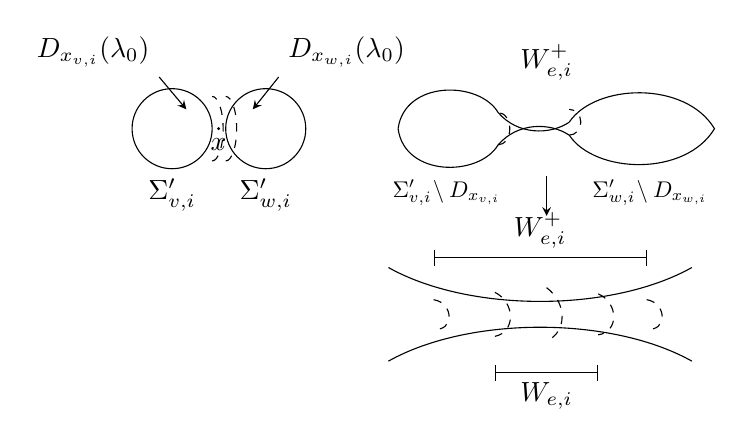
\begin{tikzpicture}[x=0.82cm,y=0.82cm,>=stealth]
 \draw (-5.70,1.45) circle (0.62) (-4.25,1.45) circle (0.62);
 \draw[dashed] (-5.08,0.95) arc[start angle=-90,end angle=90,x radius=0.17,y radius=0.50];
 \draw[dashed] (-4.87,0.95) arc[start angle=-90,end angle=90,x radius=0.17,y radius=0.50];
 \fill (-4.98,1.45) circle (0.025) node[below] {$x$};
 \node[above left] (dv) at (-5.90,2.25) {$D_{x_{v,i}}(\lambda_0)$};
 \node[above right] (dw) at (-4.05,2.25) {$D_{x_{w,i}}(\lambda_0)$};
 \draw[->] (dv.south east)--(-5.48,1.75);
 \draw[->] (dw.south west)--(-4.45,1.75);
 \node[below] at (-5.70,0.82) {$\Sigma'_{v,i}$};
 \node[below] at (-4.25,0.82) {$\Sigma'_{w,i}$};

 \draw (-2.20,1.45) .. controls (-2.10,2.20) and (-0.95,2.20) .. (-0.65,1.70)
                      .. controls (-0.35,1.35) and (0.15,1.35) .. (0.45,1.55);
 \draw (-2.20,1.45) .. controls (-2.10,0.70) and (-0.95,0.70) .. (-0.65,1.20)
                      .. controls (-0.35,1.55) and (0.15,1.55) .. (0.45,1.35);
 \draw (0.45,1.55) .. controls (0.85,2.15) and (2.25,2.20) .. (2.70,1.45)
                    .. controls (2.25,0.70) and (0.85,0.75) .. (0.45,1.35);
 \draw[dashed] (-0.65,1.20) arc[start angle=-90,end angle=90,x radius=0.18,y radius=0.25];
 \draw[dashed] (0.45,1.35) arc[start angle=-90,end angle=90,x radius=0.18,y radius=0.20];
 \node[below,scale=0.82] at (-1.45,0.78) {$\Sigma'_{v,i}\!\setminus D_{x_{v,i}}$};
 \node[below,scale=0.82] at (1.70,0.78) {$\Sigma'_{w,i}\!\setminus D_{x_{w,i}}$};
 \node[above] at (0.10,2.05) {$W_{e,i}^+$};
 \draw[->] (0.10,0.72)--(0.10,0.10);

 \draw (-2.35,-0.70) .. controls (-1.10,-1.40) and (1.10,-1.40) .. (2.35,-0.70);
 \draw (-2.35,-2.15) .. controls (-1.10,-1.45) and (1.10,-1.45) .. (2.35,-2.15);
 \foreach \x in {-1.65,-0.70,0.10,0.90,1.65}{
   \draw[dashed] (\x,{-1.00-0.12*abs(\x)}) .. controls ({\x+0.32},-1.25) and ({\x+0.32},-1.70) .. (\x,{-1.85+0.12*abs(\x)});
 }
 \draw[|-|] (-1.65,-0.55)--(1.65,-0.55) node[midway,above] {$W_{e,i}^+$};
 \draw[|-|] (-0.70,-2.33)--(0.90,-2.33) node[midway,below] {$W_{e,i}$};
\end{tikzpicture}
\caption{颈部区域。}
\label{fig:neck-region}
\end{figure}

由命题\ref{prop:derivative-bound-away-necks}，$u_i$ 在每个紧子集
$K\subset\Sigma_\infty^+\setminus\operatorname{Sing}(\Sigma_\infty^+)$ 上按
$C^\infty$ 拓扑收敛。事实上，对给定 $\mu>0$ 先选取子列，再令 $\mu\to0$ 并取
对角子列即可。最后这句话是有意义的：对任意这样的 $K$，可以选紧集
$K_i\subset\Sigma_i^+\setminus\operatorname{Sing}(\Sigma_\infty^+)$，使
$K_i\to K$，且 $(u_i,K_i)\to(u_\infty,K)$。

特别地，$u_i|_{\partial W_{e,i}^+(\lambda_0)}$ 收敛，因为 $u_i$ 在紧集
\[
 K_i=\Sigma_i^+\setminus\bigcup_eW_{e,i}^+(\lambda_0),
 \qquad
 K=\Sigma_\infty^+\setminus\bigcup_eW_{e,\infty}^+(\lambda_0)
 \subset\Sigma_\infty\setminus\operatorname{Sing}(\Sigma_\infty)
\]
上收敛。因此可在 $W_{e,i}^+(\lambda_0)$ 上重复上面用于 $W(\mu)$ 外部区域的
论证，继续增加标记点并分离气泡。取子列后，得到与 $i$ 无关的统一 $C^1$ 界
\begin{equation}
 \left|\frac{\partial u_i}{\partial\tau}\right|
 +\left|\frac{\partial u_i}{\partial t}\right|<C<\infty.
 \label{eq:uniform-derivative-bound-neck}
\end{equation}

\begin{lemma}\label{lem:small-derivative-middle-long-neck}
可以适当增加标记点、对子列取新极限并分离气泡分支，使：对每个
$\epsilon>0$，存在 $L(\epsilon)>0$ 与整数 $i(\epsilon)$，满足
\begin{enumerate}[label=(\roman*)]
 \item $L(\epsilon),i(\epsilon)\to\infty$ 当 $\epsilon\to0$；
 \item 若 $\tau\in[-L_{e,i}+L(\epsilon),L_{e,i}-L(\epsilon)]$ 且
 $i>i(\epsilon)$，则
 \[
  \left|\frac{\partial u_i}{\partial\tau}(\tau,t)\right|
  +\left|\frac{\partial u_i}{\partial t}(\tau,t)\right|\le\epsilon
 \]
 对所有 $i$ 成立。
\end{enumerate}
\end{lemma}

\begin{proof}
反设存在 $\epsilon_2>0$，使任取 $L_2\in\mathbb R$、$i_2\in\mathbb N$，都有某
$i>i_2$、$T_i\in[-L_{e,i}+L_2,L_{e,i}-L_2]$ 及 $t_i\in S^1$，满足
\[
 \left|\frac{\partial u_i}{\partial\tau}(T_i,t_i)\right|
 +\left|\frac{\partial u_i}{\partial t}(T_i,t_i)\right|\ge\epsilon_2.
\]

\begin{figure}[htbp]
\centering
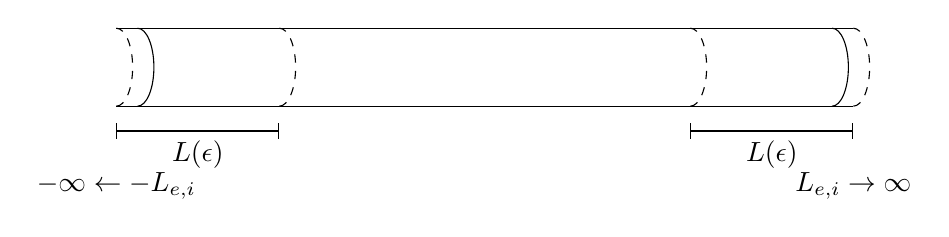
\begin{tikzpicture}[x=0.90cm,y=0.90cm,>=stealth]
 \draw (-5.2,0.55)--(5.2,0.55) (-5.2,-0.55)--(5.2,-0.55);
 \draw[dashed] (-5.2,-0.55) arc[start angle=-90,end angle=90,x radius=0.23,y radius=0.55];
 \draw (-4.90,-0.55) arc[start angle=-90,end angle=90,x radius=0.23,y radius=0.55];
 \draw[dashed] (-2.90,-0.55) arc[start angle=-90,end angle=90,x radius=0.23,y radius=0.55];
 \draw[dashed] (2.90,-0.55) arc[start angle=-90,end angle=90,x radius=0.23,y radius=0.55];
 \draw (4.90,-0.55) arc[start angle=-90,end angle=90,x radius=0.23,y radius=0.55];
 \draw[dashed] (5.2,-0.55) arc[start angle=-90,end angle=90,x radius=0.23,y radius=0.55];
 \draw[|-|] (-5.2,-0.90)--(-2.90,-0.90) node[midway,below] {$L(\epsilon)$};
 \draw[|-|] (2.90,-0.90)--(5.2,-0.90) node[midway,below] {$L(\epsilon)$};
 \node[below] at (-5.2,-1.35) {$-\infty\leftarrow -L_{e,i}$};
 \node[below] at (5.2,-1.35) {$L_{e,i}\to\infty$};
\end{tikzpicture}
\caption{长颈部。}
\label{fig:long-neck}
\end{figure}

仍用 $T_i$ 表示将圆柱平移 $T_i$ 的映射，并在 $L_2\to\infty$ 时考察
$u_i\circ T_i|_{[-L_2,L_2]\times S^1}$。由于
$T_i\in[-L_{e,i}+L_2,L_{e,i}-L_2]$ 且当 $i\to\infty$ 时
$L_{e,i}-L_2\to\infty$，最终有 $L_{e,i}-L_2>L_2$（见图\ref{fig:long-neck}）。
所以 $u_i\circ T_i$ 的定义域最终包含 $[-L_2,L_2]\times S^1$。
由\eqref{eq:uniform-derivative-bound-neck}，它在该圆柱上一致有导数界，并且
$|d(u_i\circ T_i)(0,t_i)|\ge\epsilon_2$。令 $L_2\to\infty$，便能在 $T_i$
附近为 $u_i$ 抽取一个非恒定气泡。随后在圆柱上适当地加入两个新标记点，并在
德利涅--芒福德空间中取新稳定曲线的极限；这一过程会增加 $V_1$ 中的分支数。由于
$\#V_1$ 有与新增标记点数无关的统一上界，重复有限次后即得引理。
\end{proof}

下面的引理容易证明，故留作习题。
\begin{lemma}\label{lem:diameter-decay-middle-neck}
在引理\ref{lem:small-derivative-middle-long-neck}的假设下，存在与 $i$ 无关的
$C',k'>0$，使
\[
 \operatorname{Diam}(u_i([-L_{e,i}+B,L_{e,i}-B]\times S^1))
 \le C'e^{-k'B}
\]
对所有 $0<B\le L_{e,i}-1$ 成立。
\end{lemma}

\begin{exercise}\label{ex:diameter-decay-middle-neck}
证明此引理。（提示：若 $f:\mathbb R\to\mathbb R$ 满足
$d^2f/dt^2\ge\lambda f$，$\lambda>0$，且
$|f(\pm L)|\le C_0$，则
\begin{equation}
 |f(t)|\le C_1e^{-\sqrt\lambda\operatorname{dist}(t_1\pm L)},
 \label{eq:one-dimensional-exponential-decay}
\end{equation}
其中 $t\in[-L,L]$。亦可参见命题 14.1.5 的证明。）
\end{exercise}

取 $B=L_{e,i}/2$；对一切充分大的 $i$，它当然小于 $L_{e,i}-1$。因而由引理得到
\[
 \operatorname{diam}\bigl(u_i([-L_{e,i}/2,L_{e,i}/2]\times S^1)\bigr)
 \le C'e^{-(k'/2)L_{e,i}}
\]
对所有 $i$ 成立。因此
\[
 \lim_{\mu\to0}\limsup_{i\to\infty}
 \operatorname{Diam}(u_i(W_{e,i}(\mu)))=0.
\]
结合颈外紧集上 $u_i$ 的收敛（命题 9.5.28），便得到适当新增标记点后的稳定收敛
\[
 \operatorname{s-lim}_{i\to\infty}
 [((\Sigma_i,\boldsymbol z_i^+),u_i)]
 =[((\Sigma_\infty,\boldsymbol z_\infty^+),u_\infty)].
\]

\textbf{遗忘新增标记点。}
现在移除 $\boldsymbol w_i$，回到原序列。需要定义
$\operatorname{forget}_{m+n;m}$。

\begin{definition}\label{def:dead-and-ghost-components}
\stfhIndex{I094}{si^fen^zhi}{死分支（dead component）}
\stfhIndex{I141}{you^ling^fen^zhi}{幽灵分支（ghost component）}
若 $\Sigma_\infty$ 的常值分支 $\Sigma_{\infty,v}$ 在移除全部新增辅助标记点后变得不稳定，则称为\emph{死分支}；若移除后仍稳定，则称为\emph{幽灵分支}。见图\ref{fig:dead-components}。
\end{definition}

任一死分支至多有两个奇点。考察所有死分支之并，并令
$Y=\bigcup_{l\in L}\Sigma_{\infty,v_l}$ 为它的一个连通分支；$u_\infty$ 把 $Y$
映到一点。接着考察与 $u_i$ 相伴的相应曲面之并
\[
 \bigcup_{l\in L}\left(
 \Sigma_{i,v_l}\setminus\bigcup_{x_e}D_{x_{e,i}}(\lambda_i)
 \right),
\]
并把 $Y$ 的每个奇点处的颈部重新接回，也包括 $Y$ 同邻近稳定分支相交处的颈部；
记所得开曲面为 $Y_i$。$Y_i$ 的拓扑型只能是圆盘或圆柱。若 $Y_i$ 是圆盘型，
它至多带有一个原标记点；若为环带型，则不含任何原标记点。

\begin{figure}[htbp]
\centering
\setlength{\unitlength}{0.8mm}
\begin{picture}(125,28)
 \put(5,14){\oval(22,16)} \put(5,14){\makebox(0,0){稳定}}
 \put(24,14){\oval(20,12)} \put(42,14){\oval(20,12)}
 \put(60,14){\oval(20,12)} \put(82,14){\oval(24,18)}
 \put(82,14){\makebox(0,0){死分支}}
 \put(25,2){\line(1,0){38}} \put(25,0){\line(0,1){4}}
 \put(63,0){\line(0,1){4}} \put(44,-3){\makebox(0,0){$D$}}
 \put(44,24){\makebox(0,0){$Y_i$}}
\end{picture}
\caption{死分支。}
\label{fig:dead-components}
\end{figure}

从 $Y_i$ 移除全部新增标记点。已知
$\operatorname{Diam}(u_i(Y_i))\to0$，由上述考虑可知所得预稳定映射是稳定的。
记所得稳定映射为 $((\Sigma_i,\boldsymbol z_i^{+-}),u_i)$。再从
$Y\subset\Sigma_\infty$ 中移除所有新增标记点，收缩 $Y$ 的全部分支，并记所得稳定映射为
$((\Sigma_\infty,\boldsymbol z_\infty^{+-}),u_\infty)$。

随后可安全地从稳定映射
\[
 ((\Sigma_\infty,\boldsymbol z_\infty^{+-}),u_\infty)
\]
的非恒定分支上移除所有新增标记点，并相应地从
$((\Sigma_i,\boldsymbol z_i^{+-}),u_i)$ 上移除这些点。分别记所得稳定映射为
\[
 ((\Sigma_\infty,\boldsymbol z_\infty^{+--}),u_\infty),
 \qquad ((\Sigma_i,\boldsymbol z_i^{+--}),u_i).
\]
由构造，前者属于相应的稳定映射空间，而
\[
 [((\Sigma_i,\boldsymbol z_i^{+--}),u_i)]
 =[((\Sigma_i,\boldsymbol z_i),u_i)].
\]
于是显然有
\[
 \operatorname{forget}_{m+n;m}
 [((\Sigma_i,\boldsymbol z_i^+),u_i)]
 =[((\Sigma_i,\boldsymbol z_i),u_i)],
\]
并且
\[
 \operatorname{forget}_{m+n;m}
 [((\Sigma_\infty^+,\boldsymbol z_\infty^+),u_\infty)]
 =[((\Sigma_\infty,\boldsymbol z_\infty^{+--}),u_\infty)]
\]
在 $\overline{\mathcal M}_{g,m}(M,J;\beta)$ 中良定。故按
定义\ref{def:general-stable-map-convergence}，
\[
 \lim_{i\to\infty}[((\Sigma_i,\boldsymbol z_i),u_i)]
 =[((\Sigma_\infty,\boldsymbol z_\infty^{+--}),u_\infty)].
\]
这最终完成紧性的证明。

\subsection{豪斯多夫性}
\stfhSubIndexRangeEnd{I261}{wen^ding^ying^she^ta^pu}{稳定映射拓扑（stable map topology）}{jin^xing}{紧性（compactness）}
\label{subsec:stable-map-hausdorff-property}
\stfhSubIndexRangeStart{I263}{wen^ding^ying^she^ta^pu}{稳定映射拓扑（stable map topology）}{hao^si^duo^fu^xing^zhi}{豪斯多夫性质（Hausdorff property）}

回忆遗忘映射
\[
 \operatorname{forget}_{m+n;m}:
 \overline{\mathcal M}_{g,m+n}(M,J;\beta)
 \longrightarrow\overline{\mathcal M}_{g,m}(M,J;\beta).
\]
遗忘末 $n$ 个标记点后，若某不可约分支亏格为零、其上映射恒定且变得不稳定，就把它收缩为一点；若仍稳定，则只删除指定标记点。

\begin{theorem}\label{thm:stable-map-topology-hausdorff}
$\overline{\mathcal M}_{g,m}(M,J;\beta)$ 上的稳定映射拓扑是豪斯多夫的。
\end{theorem}

\begin{proof}
为了证明豪斯多夫性，必须证明
$\overline{\mathcal M}_{g,m}(M,J;\beta)\times
\overline{\mathcal M}_{g,m}(M,J;\beta)$ 的对角集是闭集。回忆稳定映射集合
$\widetilde{\mathcal M}_{g,m}(M,J;\beta)$ 可度量化，因而证明下述断言便已足够。

设 $((\Sigma_i,\boldsymbol z_i),u_i)$、
$((\Sigma_i',\boldsymbol z_i'),u_i')\in
\widetilde{\mathcal M}_{g,m}(M,J;\beta)$ 是稳定映射中一个收敛等价类序列的两组代表，
即
\[
 [((\Sigma_i,\boldsymbol z_i),u_i)]
 =[((\Sigma_i',\boldsymbol z_i'),u_i')].
\]
依稳定映射拓扑中收敛的定义，存在定义域的稳定化
$(\Sigma_i,\boldsymbol z_i^+)$ 与
$(\Sigma_i',\boldsymbol z_i^{\prime+})$，使
\[
 \operatorname{s-lim}_{i\to\infty}[((\Sigma_i,\boldsymbol z_i^+),u_i)]
 =[((\Sigma_\infty,\boldsymbol z_\infty^+),u_\infty)]
 \quad\text{于 }\overline{\mathcal M}_{g,m+n}^{st}(M,J;\beta),
\]
以及
\[
 \operatorname{s-lim}_{i\to\infty}
 [((\Sigma_i',\boldsymbol z_i^{\prime+}),u_i')]
 =[((\Sigma_\infty',\boldsymbol z_\infty^{\prime+}),u_\infty')]
 \quad\text{于 }\overline{\mathcal M}_{g,m+n'}^{st}(M,J;\beta).
\]
同时
\[
 [((\Sigma,\boldsymbol z),u)]
 =\operatorname{forget}_{m+n;m}
 [((\Sigma_\infty,\boldsymbol z_\infty^+),u_\infty)],
\]
\[
 [((\Sigma',\boldsymbol z'),u')]
 =\operatorname{forget}_{m+n';m}
 [((\Sigma_\infty',\boldsymbol z_\infty^{\prime+}),u_\infty')].
\]
由定义\ref{def:general-stable-map-convergence}意义下的收敛假设，这两个表达式良定；
我们需要证明两个稳定映射 $((\Sigma,\boldsymbol z),u)$ 与
$((\Sigma',\boldsymbol z'),u')$ 同构。

由等价类定义，每个 $i$ 有双全纯映射
$\phi_i:(\Sigma_i,\boldsymbol z_i)\to(\Sigma_i',\boldsymbol z_i')$，使
$u_i'=u_i\circ\phi_i^{-1}$。在 $\Sigma_i$ 上考虑新增标记点集合
\[
 \boldsymbol z_i''=\boldsymbol z_i^+\cup\boldsymbol z_i^{\prime+}\subset\Sigma_i,
 \qquad
 \boldsymbol z_i''=\{\boldsymbol z_i,
 \boldsymbol z_i^+\setminus\boldsymbol z_i,
 \boldsymbol z_i^{\prime+}\setminus\boldsymbol z_i'\}.
\]
必要时微扰 $\boldsymbol z_i^{\prime+}\setminus\boldsymbol z_i'$ 中的点，可设
$\boldsymbol z_i''$ 中各点彼此不同。于是
$((\Sigma_i,\boldsymbol z_i''),u_i)$ 的定义域稳定，并定义
$\overline{\mathcal M}_{g,m+n+n'}^{st}(M,J;\beta)$ 中的元素。由
$\overline{\mathcal M}_{g,m+n+n'}(M,J;\beta)$ 的紧性及其拓扑定义，可再加入
$n''$ 个标记点并在必要时取子列，使
\begin{equation}
 \operatorname{s-lim}_{i\to\infty}
 [((\Sigma_i,\boldsymbol z_i''),u_i)]
 =[((\Sigma_\infty'',\boldsymbol z_\infty''),u_\infty'')].
 \label{eq:common-stabilization-limit}
\end{equation}
必要时选取子列后，对某个
$[((\Sigma_\infty,\boldsymbol z_\infty''),u_\infty)]
\in\overline{\mathcal M}_{g,m+n+n'+n''}^{st}(M,J;\beta)$，上述收敛成立。

由构造有
\[
 \operatorname{forget}_{m+n+n'+n'';m+n}
 [((\Sigma_i,\boldsymbol z_i''),u_i)]
 =[((\Sigma_i,\boldsymbol z_i^+),u_i)].
\]
收敛\eqref{eq:common-stabilization-limit}特别保证充分大的 $i$ 上各标记点一致分离。
还回忆到
\[
 \operatorname{s-lim}_{i\to\infty}
 [((\Sigma_i,\boldsymbol z_i^+),u_i)]
 =[((\Sigma_\infty,\boldsymbol z_\infty^+),u_\infty)].
\]
类似地，
\[
 \operatorname{forget}_{m+n+n'+n'';m+n'}
 [((\Sigma_i,\boldsymbol z_i''),u_i)]
 =[((\Sigma_i',\boldsymbol z_i^{\prime+}),u_i')],
\]
且
\[
 \operatorname{s-lim}_{i\to\infty}
 [((\Sigma_i',\boldsymbol z_i^{\prime+}),u_i')]
 =[((\Sigma_\infty',\boldsymbol z_\infty^{\prime+}),u_\infty')].
\]
由此分别得到
\[
 \operatorname{forget}_{m+n+n'+n'';m+n}
 [((\Sigma_\infty'',\boldsymbol z_\infty''),u_\infty'')]
 =[((\Sigma_\infty,\boldsymbol z_\infty^+),u_\infty)],
\]
\[
 \operatorname{forget}_{m+n+n'+n'';m+n'}
 [((\Sigma_\infty'',\boldsymbol z_\infty''),u_\infty'')]
 =[((\Sigma_\infty',\boldsymbol z_\infty^{\prime+}),u_\infty')].
\]
另一方面已有两个候选极限的定义式。因此
\[
 [((\Sigma,\boldsymbol z),u)]
 =\operatorname{forget}_{m+n;m}\circ
 \operatorname{forget}_{m+n+n'+n'';m+n}
 [((\Sigma_\infty'',\boldsymbol z_\infty''),u_\infty'')],
\]
并且
\[
 [((\Sigma',\boldsymbol z'),u')]
 =\operatorname{forget}_{m+n';m}\circ
 \operatorname{forget}_{m+n+n'+n'';m+n'}
 [((\Sigma_\infty'',\boldsymbol z_\infty''),u_\infty'')].
\]

\begin{lemma}\label{lem:composition-forgetful-stable-maps}
对任意 $a,b,c\in\mathbb N$，在
$\overline{\mathcal M}_{g,a+b+c}(M,J;\beta)$ 上有
\[
 \operatorname{forget}_{a+b;a}\circ
 \operatorname{forget}_{a+b+c;a+b}
 =\operatorname{forget}_{a+b+c;a}.
\]
\end{lemma}

把这个引理分别以 $(a,b,c)=(m,n,n'+n'')$ 与
$(a,b,c)=(m,n',n+n'')$ 应用于引理正上方两个等式的右端。两者都是从同一个稳定映射
$[((\Sigma_\infty'',\boldsymbol z_\infty''),u_\infty'')]
\in\overline{\mathcal M}_{g,m+n+n'+n''}(M,J;\beta)$ 中遗忘同样编号的标记点得到，
所以
$[((\Sigma,\boldsymbol z),u)]=[((\Sigma',\boldsymbol z'),u')]$，对角集闭，豪斯多夫性得证。
\stfhSubIndexRangeEnd{I263}{wen^ding^ying^she^ta^pu}{稳定映射拓扑（stable map topology）}{hao^si^duo^fu^xing^zhi}{豪斯多夫性质（Hausdorff property）}
\end{proof}
